\documentclass{article}
\usepackage{t1enc}

\usepackage[hungarian]{babel}
\usepackage[utf8]{inputenc}
\usepackage[T1]{fontenc}

\usepackage{graphicx}
\usepackage{geometry}

\usepackage{setspace}
\onehalfspacing

\usepackage{titling}
\usepackage{indentfirst}

\usepackage{xcolor}
\usepackage{graphicx} 
\usepackage{float}
\usepackage{listings}


\lstdefinelanguage{JavaScript}{
  keywords={break, case, catch, continue, debugger, default, delete, do, else, finally, for, function, if, in, instanceof, new, return, switch, this, throw, try, typeof, var, void, while, with, let, const},
  keywordstyle=\color{blue}\bfseries,
  ndkeywords={class, export, boolean, throw, implements, import, this},
  ndkeywordstyle=\color{darkgray}\bfseries,
  identifierstyle=\color{black},
  sensitive=false,
  comment=[l]{//},
  morecomment=[s]{/*}{*/},
  commentstyle=\color{gray}\ttfamily,
  stringstyle=\color{red}\ttfamily,
  morestring=[b]',
  morestring=[b]"
}

\lstset{
  backgroundcolor=\color{white!10},
  basicstyle=\ttfamily\small,
  frame=none
  language=JavaScript
}




\begin{document}

\pagestyle{plain}


\begin{titlepage}
    \centering
    \vspace*{2cm}

    {\Large \textbf{SAPIENTIA ERDÉLYI MAGYAR}}\\[0.2cm]
    {\Large \textbf{TUDOMÁNYEGYETEM}}\\[0.5cm]
    {\large MAROSVÁSÁRHELYI KAR}\\[0.2cm]
    {\large SZÁMÍTÁSTECHNIKA SZAK}\\[3cm]

    {\LARGE \textbf{PROJECT TITLE GOES HERE}}\\[0.5cm] 
    {\Large \textbf{DIPLOMADOLGOZAT}}\\[4cm]

    \begin{flushleft}
        \begin{minipage}{0.45\textwidth}
            \textbf{Témavezető:}\\
            \\
            Conf. Dr. Iclănzan Andrei David\\
        \end{minipage}
        \hfill
        \begin{minipage}{0.45\textwidth}
            \textbf{Végzős hallgató:}\\
            \\
            Szabó Huba
        \end{minipage}
    \end{flushleft}

    \vfill

    {\large Marosvásárhely, 2025}

\end{titlepage}

\begin{titlepage}
    \centering
    \vspace*{2cm}

    {\Large \textbf{UNIVERSITATEA „SAPIENTIA” DIN CLUJ-NAPOCA}}\\[0.2cm]
    {\Large \textbf{FACULTATEA DE ȘTIINȚE TEHNICE ȘI UMANISTE,}}\\[0.5cm]
    {\large TÎRGU-MUREȘ}\\[0.2cm]
    {\large  SPECIALIZAREA CALCULATOARE}\\[3cm]

    {\LARGE \textbf{DEZVOLTAREA UNEI APLICAȚII WEB DE GESTIONARE ȘI REZERVARE A BILETELOR PENTRU O FIRMĂ DE TRANSPORT}}\\[4cm] 
    

    \noindent
\begin{minipage}[t]{0.48\textwidth}
    \raggedright
    \textbf{Coordonator științific:}\\[1em]
    Conf. Dr. Iclănzan Andrei David
\end{minipage}
\hfill
\begin{minipage}[t]{0.48\textwidth}
    \raggedleft
    \textbf{Absolvent:}\\[1em]
    Szabó Huba
\end{minipage}


    \vfill

    {\large  Târgu-Mureș, 2025}

\end{titlepage}

\section*{Kivonat}

    A dolgozat célja egy valós idejű menetrendkezelő rendszer tervezése és megvalósítása, amely lehetővé teszi a
    felhasználók számára a tömegközlekedési járatok hatékony nyomon követését. A rendszer egy webes alkalmazás formájában valósul meg, amely a megállók, járatok és menetrendek adatainak kezelését, megjelenítését és jegyfoglalást is támogatja.

A dolgozat bemutatja az alkalmazás funkcionalitásait, az adatszerkezet kialakítását, a felhasznált technológiákat (például ASP.NET Core MVC, Entity Framework, Google Maps API), valamint a fejlesztés során felmerült kihívásokat és azok megoldásait.

A rendszer célja, hogy segítse a felhasználókat a gyors és egyszerű információelérésben, továbbá növelje a közösségi közlekedés használhatóságát és hatékonyságát.

\vspace{1cm}

\noindent\textbf{Kulcsszavak:} menetrend, tömegközlekedés, ASP.NET, térkép, webalkalmazás

\section*{Abstract}

Scopul acestei lucrări este proiectarea și implementarea unui sistem de gestionare a orarelor în timp real, care să permită utilizatorilor urmărirea eficientă a mijloacelor de transport public. Sistemul este realizat sub forma unei aplicații web, care sprijină gestionarea, afișarea și rezervarea datelor legate de stații, rute și orare.

Lucrarea prezintă funcționalitățile aplicației, structura de date utilizată, tehnologiile folosite (de exemplu ASP.NET Core MVC, Entity Framework, Google Maps API), precum și provocările întâlnite în timpul dezvoltării și soluțiile adoptate.

Scopul sistemului este de a sprijini utilizatorii în accesarea rapidă și ușoară a informațiilor, precum și de a îmbunătăți utilizabilitatea și eficiența transportului public.

\vspace{1cm}

\noindent\textbf{Cuvinte cheie:} orar, transport public, ASP.NET, hartă, aplicație web


\tableofcontents
\newpage
\section{Bevezetés}

\indent A mai rohanó világban egyre többen választják az autót a tömegközlekedés helyett. Személy szerint mindig is a tömegközlekedést részesítettem előnyben, ha tehettem – kényelmesebb, fenntarthatóbb megoldás, és sokszor olcsóbb is, mint autóval közlekedni. Ugyanakkor számos alkalommal szembesültem azzal, hogy a buszközlekedés nem mindig olyan egyszerű, mint amilyennek elsőre tűnik. Például Marosvásárhelyen több ízben is hosszú időt töltöttem azzal, hogy rájöjjek, egy adott járat pontosan honnan indul, hol áll meg, és hogyan jutok el egyik pontról a másikra.

Gyakran előfordult, hogy a buszmegállók nevei nem egyeztek az utcák nevével, így a térképen sem lehetett őket pontosan beazonosítani. Ráadásul az útvonalak sokszor nincsenek térképesen megjelenítve, és a menetrendek is nehezen értelmezhetőek. A legtöbb online elérhető felület túlzsúfolt, nem felhasználóbarát, így ahelyett, hogy segítséget nyújtana, inkább további zavart kelt.

Ezek a személyes tapasztalatok ösztönöztek arra, hogy elindítsam ezt a projektet, amelynek célja egy olyan webes alkalmazás megalkotása, amely segít a felhasználóknak eligazodni a buszközlekedés világában. A rendszer egyszerű, letisztult kezelőfelületet biztosít, és térképes nézettel segíti a járatok és útvonalak átláthatóságát.

A fejlesztés során nemcsak az utasokra gondoltam, hanem a szolgáltatók, például a sofőrök, diszpécserek és céges adminisztrátorok igényeit is figyelembe vettem. Mivel régóta érdekel a vállalatirányítás és az ügyfélkapcsolat-kezelés (CRM), fontosnak tartottam olyan funkciók beépítését is, amelyek támogatják a belső munkafolyamatokat, és hatékonyabbá teszik a szervezeti működést.

A projekt webes felületen működik, mivel napjainkban ez a legelérhetőbb és legpraktikusabb forma a felhasználók számára. A .NET technológia mellett döntöttem, mivel számos modern funkcióval, stabil háttérrel és vizuálisan igényes UI csomaggal rendelkezik, amelyekkel öröm dolgozni. A rendszer így nemcsak funkcionálisan, hanem megjelenésében is a mai igényekhez igazodik.

Végezetül fontosnak tartom megjegyezni, hogy ez a projekt nem egy lezárt megoldás, hanem egy olyan alap, amely később számos irányba továbbfejleszthető. Legyen szó mobilalkalmazásról, mesterséges intelligencia alapú útvonaltervezésről vagy mélyebb CRM-rendszer beépítéséről, a lehetőségek széles skálája áll nyitva.


\newpage
%% ASP.NET MVC Architecture

\section{ASP.NET MVC architektúra}

\indent Az államvizsga-dolgozatom célja bemutatni egy webalapú alkalmazás fejlesztési folyamatát és technológiai hátterét, amely egy buszvállalat működését támogatja. A fejlesztés során az ASP.NET MVC keretrendszerre építek, amely jól strukturált megközelítést kínál a webes alkalmazások építéséhez, miközben lehetővé teszi az üzleti logika, a megjelenítés és az adatkezelés hatékony szétválasztását.

A dolgozat első fejezete a .NET platform által kínált lehetőségekre és az MVC (Model-View-Controller) architektúra alapelveire összpontosít. Részletesen ismertetjük a modell, a nézet és a vezérlő szerepét, valamint ezek együttműködését a rendszer működésében. Külön figyelmet fordítunk az útvonalkezelés és az adatátadás mechanizmusaira is, amelyek az ASP.NET MVC egyik kulcsfontosságú komponensét jelentik.

A következő alfejezetekben bemutatásra kerülnek azok a technológiák, amelyek kiegészítik és támogatják az alkalmazás működését. Az Entity Framework révén az adatbázis-kezelés objektumorientált módon valósul meg, míg a Razor nézetmotor a dinamikus tartalmak hatékony megjelenítését teszi lehetővé. A kliensoldali működéshez elengedhetetlen JavaScript mellett a Leaflet könyvtár térképes vizualizációt biztosít, amely különösen hasznos a szállítási útvonalak megjelenítéséhez. A rendszer részeként implementált e-mail értesítések SMTP protokollon keresztül működnek, míg a QR-kód generálás lehetőséget nyújt például jegyek, csomagazonosítók vagy beléptetési információk digitális tárolására és gyors elérésére.

\begin{figure}[H]
    \centering
    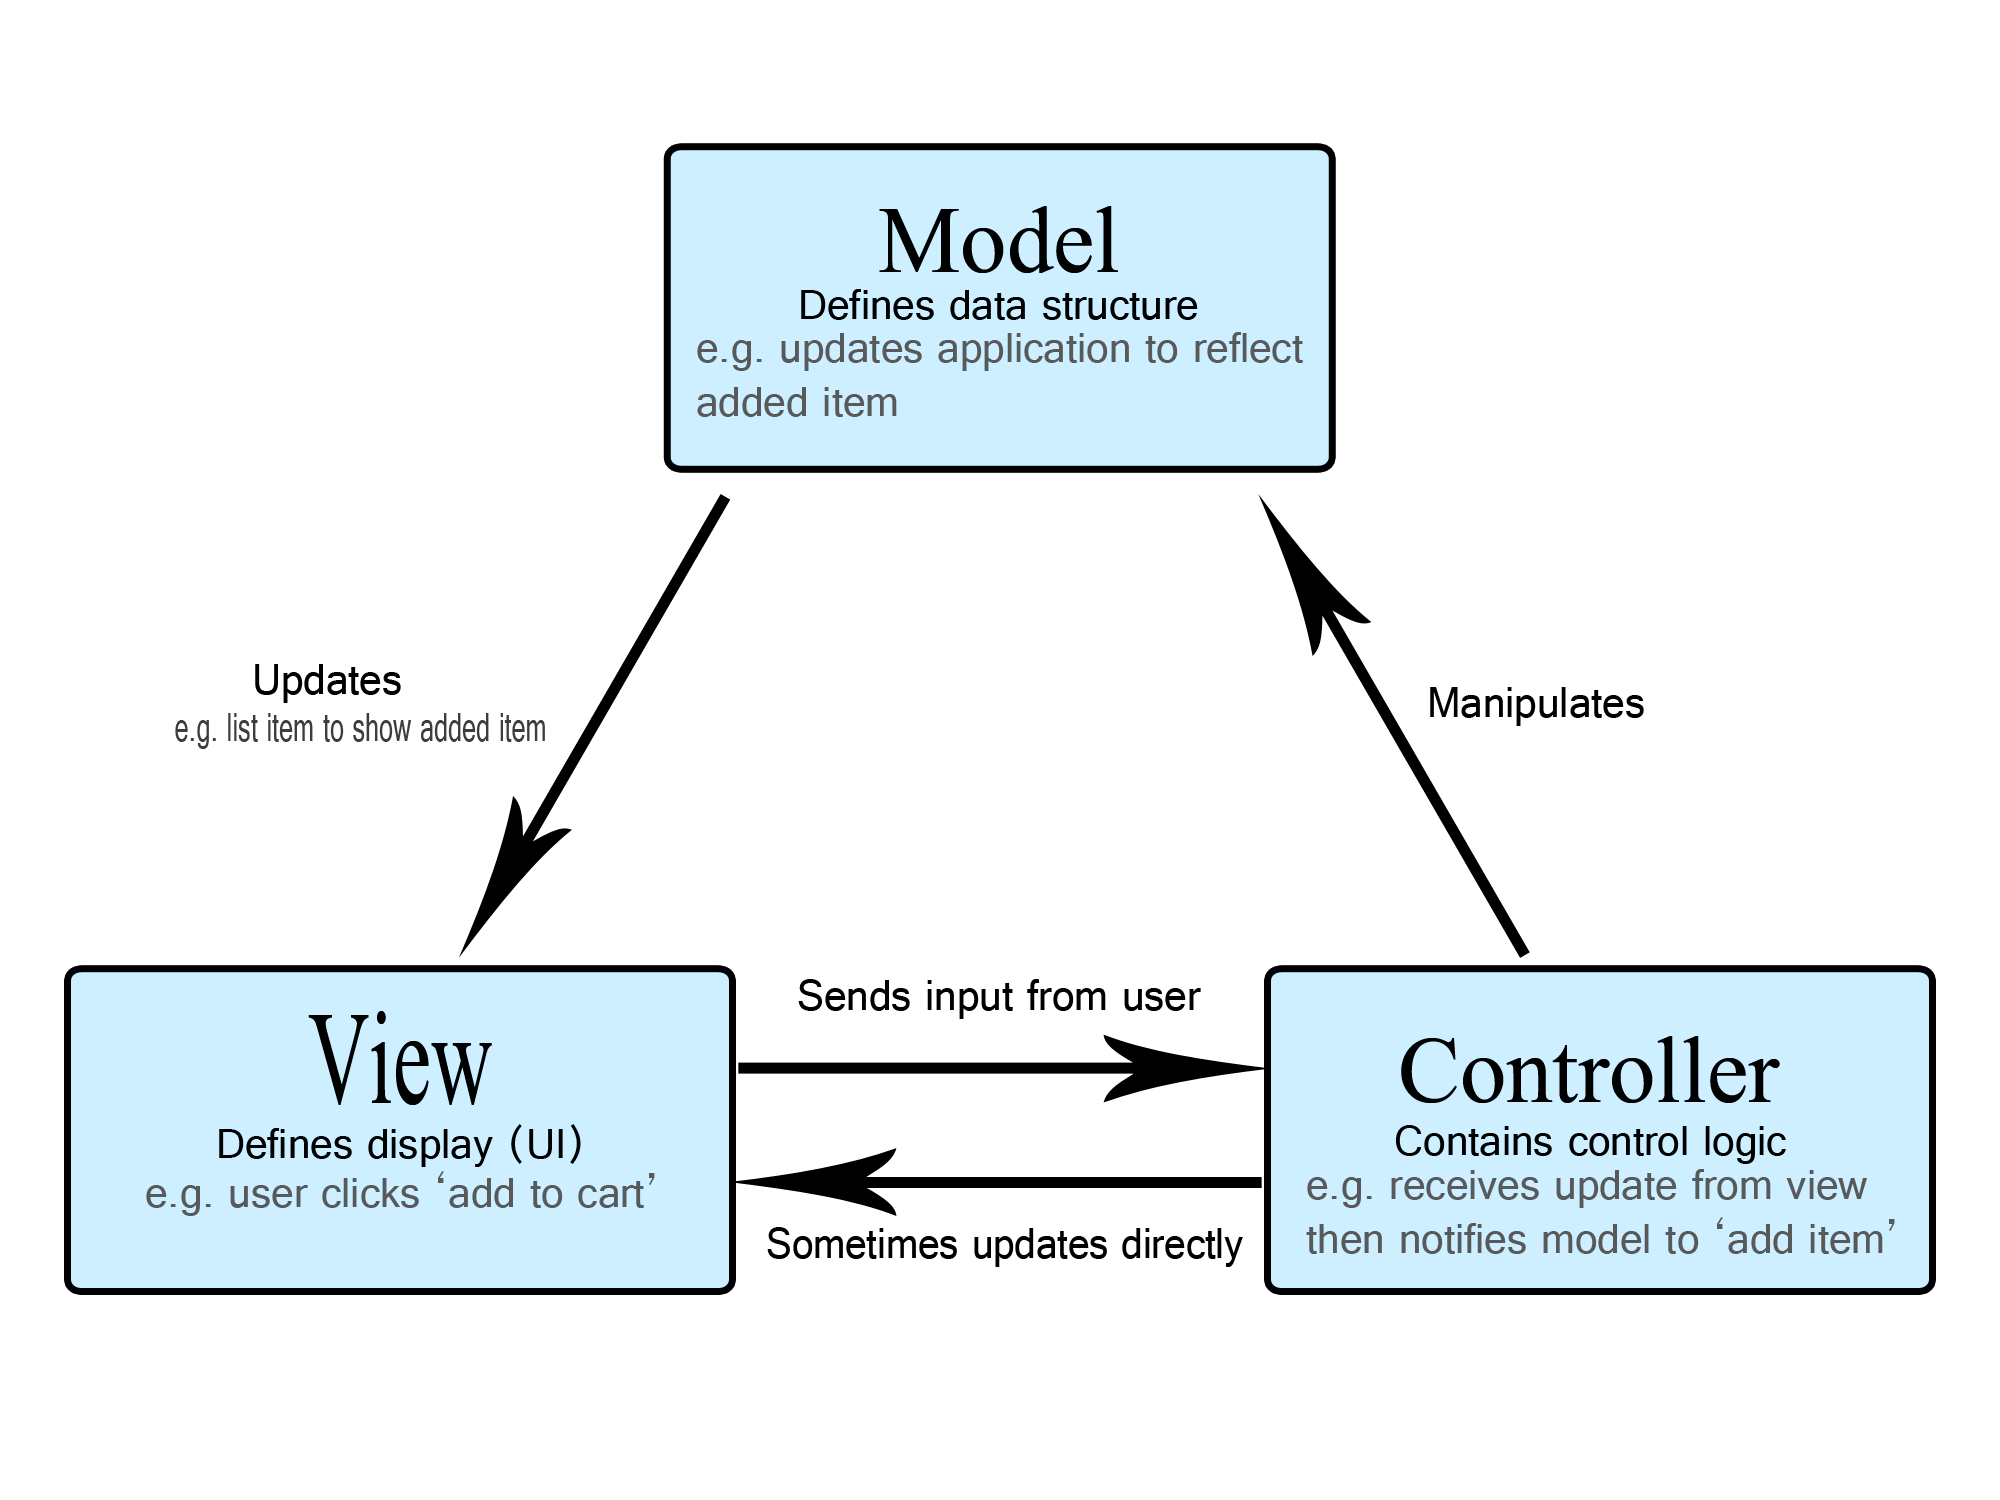
\includegraphics[width=1\textwidth]{Szakdolgozat/Mellekletek/model-view-controller-light-blue.png}
    \caption{Az MVC (Model–View–Controller) architektúra felépítése. Az ábrán jól látható, hogyan különül el az adatkezelés (Model), a felhasználói felület (View) és az üzleti logikát kezelő vezérlő (Controller). Az egyes rétegek közötti kommunikáció segíti az alkalmazás moduláris, karbantartható és tesztelhető kialakítását. (Forrás: MVC Architektúra – MDN Web Docs)}
    \label{fig:er-diagram}
\end{figure}


\subsection{A .NET platform és az MVC minta}

\indent A .NET egy többnyelvű, keresztplatformos fejlesztési környezet, amelyet a Microsoft hozott létre, és amely lehetőséget nyújt különböző típusú alkalmazások – például asztali, webes és mobil – fejlesztésére. A platform célja, hogy egységes, megbízható és jól skálázható környezetet biztosítson a fejlesztők számára. Ezen belül az ASP.NET a webalkalmazások készítésére szolgáló keretrendszer, amely támogatja az MVC (Model–View–Controller) mintát.

Az MVC architektúra egyik legfontosabb előnye az alkalmazás logikájának, adatainak és felhasználói felületének elkülönítése. Ez nemcsak a kód tisztaságát és átláthatóságát javítja, hanem lehetővé teszi a különböző fejlesztői szerepkörök (pl. backend, frontend) hatékony együttműködését, valamint a rendszer egyszerűbb tesztelhetőségét és karbantarthatóságát.

\subsubsection{ASP.NET MVC alapelvei}

\indent Az ASP.NET MVC keretrendszer három jól elkülöníthető rétegre bontja az alkalmazás struktúráját. A Model réteg felelős az üzleti logika és az adatok kezeléséért, a View a felhasználó számára megjelenített tartalmat írja le, míg a Controller a két réteg közötti kommunikációért és az események kezeléséért felel. Ez az elkülönítés elősegíti az egységek külön történő fejlesztését és tesztelését.

Az ASP.NET MVC a REST architektúra alapelveit követi, és szorosan épít az URL-alapú útvonalkezelésre (routing), amely meghatározza, hogy egy adott kérés melyik vezérlőhöz és metódushoz kerüljön.

\subsubsection{A Controller, View és Model szerepe}

\indent A Controller felelős a beérkező HTTP-kérések kezeléséért, az adatok lekérdezéséért vagy módosításáért, és végül az adatok továbbításáért a View felé. A Model tartalmazza az alkalmazás által kezelt adatokat és azok viselkedését, gyakran adatbázissal kapcsolatban álló entitások és azok logikája formájában. A View Razor szintaxisban írt .cshtml fájlokat jelent, amelyek HTML-ben jelenítik meg a Modelből származó adatokat, ezzel biztosítva a dinamikus tartalom megjelenítését.

\subsubsection{Routing és adatátadás}

\indent Az útvonalkezelés (routing) kulcsszerepet játszik az ASP.NET MVC működésében. Az URL-ek mintákat követnek, amelyek alapján a rendszer eldönti, hogy melyik Controller és azon belül melyik Action metódus hajtódjon végre. Az adatok átadása történhet route paramétereken, query stringen vagy formokon keresztül, míg az adatok feldolgozását és továbbítását a Controller végzi, amely továbbküldi azokat a View vagy más üzleti logikai rétegek számára.

\subsection{Kapcsolódó technológiák}

\subsubsection{Entity Framework és az adatkezelés integrációja}

\indent Az Entity Framework (EF) a .NET keretrendszer objektum-relációs leképezést (ORM) alkalmazó technológiája, amely lehetővé teszi, hogy az adatbázis-műveleteket magas szintű, típusosan definiált C\# osztályokon keresztül végezzük el. Az EF célja, hogy a relációs adatbázisokkal való munka során elrejtse a nyers SQL lekérdezések szükségességét, ezáltal elősegítve a biztonságosabb és karbantarthatóbb adatkezelést.

Az EF támogatja a különböző adatmodellezési megközelítéseket, köztük a Code First és Database First stratégiákat. A Code First megközelítés lehetővé teszi, hogy a fejlesztők először az osztálystruktúrát hozzák létre a C\# nyelv eszközeivel, majd az EF automatikusan létrehozza és karbantartja a hozzá tartozó adatbázis-sémát. Ezzel szemben a Database First modell olyan helyzetekben előnyös, ahol már létező adatbázis-struktúrához kell alkalmazkodni.

Az alkalmazás adatbázis-kommunikációja általában Microsoft SQL Serverrel történik, amely a .NET ökoszisztémán belül natívan támogatott. Az EF SQL Serverrel való összekapcsolását a DbContext konfigurálásán keresztül végezzük, ahol a kapcsolat elérési adatai (connection string) egy konfigurációs fájlban vagy programkódban definiálhatók. A kapcsolat biztonságos kezeléséhez jellemzően Windows hitelesítést vagy SQL Server hitelesítést használunk, opcionálisan SSL titkosítással.

A modern ASP.NET alapú alkalmazásokban az EF szorosan együttműködik az ASP.NET Identity keretrendszerrel, amely a felhasználókezelési és hitelesítési feladatokat látja el. Az Identity rendszer szintén az EF-en keresztül valósítja meg a felhasználói adatok (pl. regisztrációs információk, jelszavak hash-elve, jogosultságok, szerepkörök) tartós tárolását és kezelését. A felhasználói entitások a többi modellosztályhoz hasonlóan entitásként jelennek meg az adatbázisban, így az EF által biztosított LINQ-lekérdezések és migrációs eszközök teljes mértékben alkalmazhatók rájuk is.

Ez az integrált megközelítés lehetővé teszi, hogy az alkalmazás egységes módon kezelje mind az üzleti, mind az autentikációs adatokat, miközben biztosítja az adatbázis-struktúra automatikus frissítését és bővítését a fejlesztés során.

\subsubsection{Razor nézetek}

\indent A Razor egy modern, egyszerű szintaxisú nézetmotor, amely a HTML és C\# nyelv elemeit ötvözi. Lehetővé teszi, hogy a dinamikus tartalom hatékonyan jelenjen meg a felhasználói felületen, miközben a kód jól olvasható marad. A Razor nézetek általában {.cshtml} kiterjesztésű fájlokban jelennek meg, és az alkalmazás prezentációs rétegének meghatározó elemei.

\indent A megjelenítés esztétikai és felhasználói élménybeli szempontból történő javítása érdekében a Razor nézetekben gyakran alkalmazzák a Bootstrap keretrendszert, amely előre definiált, reszponzív stílusokat és elrendezéseket kínál. Emellett elterjedt a Bootstrap Icons (BI) használata is, amely vektor alapú ikonokat biztosít a vizuális elemek kiegészítésére és gazdagítására. Ezen eszközök integrálása nemcsak a fejlesztési folyamatot gyorsítja fel, hanem hozzájárul a konzisztens és professzionális megjelenés kialakításához is.



\subsubsection{JavaScript és front-end integráció}

\indent A JavaScript a modern webfejlesztés alapköve, amely biztosítja az interaktív felhasználói élményt. ASP.NET MVC alkalmazásokban jellemzően jQuery, AJAX vagy más könyvtárak és keretrendszerek is helyet kapnak, hogy lehetővé tegyék az aszinkron adatkommunikációt és a kliensoldali eseménykezelést.

\subsubsection{Leaflet}

\indent A Leaflet egy könnyű, nyílt forráskódú JavaScript könyvtár, amely interaktív térképek megjelenítését teszi lehetővé. A könyvtár különösen alkalmas útvonalak, megállók és helymeghatározások vizualizálására, így jól illeszkedik logisztikai vagy közlekedési célú alkalmazásokba.

\subsubsection{E-mailküldés SMTP protokollal}

\indent A levelezési funkciók megvalósításához az ASP.NET alkalmazásokban a .NET beépített System.Net.Mail névtere használható, amely támogatja az SMTP-alapú üzenetküldést. A konfiguráció során megadható a szerver címe, a hitelesítéshez szükséges adatok, valamint biztonságos (SSL/TLS) kapcsolódási lehetőségek. Ez lehetővé teszi automatikus értesítések, regisztrációs visszaigazolások vagy tranzakciós levelek küldését.

\subsubsection{QR-kód generálás}

\indent A QR-kódok lehetővé teszik különböző típusú információ gyors és vizuálisan is feldolgozható ábrázolását. ASP.NET MVC alkalmazásokban a QRCoder könyvtár használatával könnyen létrehozhatók ilyen kódok, amelyek tartalmazhatnak URL-eket, azonosítókat vagy bármilyen szöveges adatot, például jegyek, csomagazonosítók vagy belépési információk formájában.




\newpage
\section{Rendszerkövetelmények}

\subsection{Funkcionális és nem-funkcionális követelmények}

\indent Az alkalmazás fejlesztésének egyik legfontosabb kiindulópontja a világos és egyértelmű követelményrendszer meghatározása. A követelmények két fő kategóriába sorolhatók: funkcionális és nem-funkcionális követelmények. 

\subsection{Funkcionális követelmények}

A funkcionális követelmények azokat az elvárt viselkedéseket és szolgáltatásokat írják le, amelyeket a rendszernek teljesítenie kell. Ide tartoznak például a felhasználók által végrehajtható műveletek, az adatfolyamatok, valamint a rendszer reakciói különféle eseményekre vagy bemenetekre. A funkcionális követelmények meghatározzák, hogy mit csinál a rendszer, és ezek képezik az alapját a fejlesztési és tesztelési folyamatoknak.


\subsubsection{Contact}

A \textit{Contact} modell az alkalmazás felhasználóit reprezentálja, és lehetővé teszi a regisztráció, bejelentkezés, valamint a felhasználói adatok kezelésének funkcióit. A rendszer támogatja különböző szerepkörök (utas, sofőr, adminisztrátor) hozzárendelését a felhasználókhoz, amely szerepek befolyásolják a hozzáférési jogosultságokat. A felhasználók személyes adatai – beleértve a nevet, lakcímet és irányítószámot – utólag is módosíthatók a profilkezelő felületen keresztül. Az adminisztrátor jogosult egyes felhasználók inaktiválására is, amely funkció különösen hasznos a visszaélések vagy szabálytalanságok esetén történő fiókletiltás során.



\subsubsection{Ticket}

A \textit{Ticket} entitás a rendszerben megvásárolt jegyeket írja le, és szoros kapcsolatban áll a menetrendi adatokkal, valamint a felhasználói profillal. Jegyvásárlás során a rendszer automatikusan hozzárendel egy szabad ülőhelyet a kiválasztott járathoz. A tranzakció befejeztével a felhasználó egy automatikusan generált visszaigazoló e-mailt kap, amelyhez mellékletként QR-kód is csatolásra kerül.

Ez a QR-kód hordozza a legfontosabb utazási információkat, például a járatszámot, az indulási és érkezési állomásokat, valamint az útvonal teljes menetidejét. A felhasználó ezenkívül a \textit{Ticket Detail} nézeten keresztül részletesen is megtekintheti a jegyhez kapcsolódó adatokat – ideértve az indulás és érkezés időpontját, az utazási vonalat, valamint a kijelölt ülőhelyet.

A felület egy interaktív térképet is tartalmaz, amely grafikus formában mutatja be az adott utazás útvonalát. Fontos megjegyezni, hogy a QR-kód nem a jegyoldalon jelenik meg, hanem kizárólag a visszaigazoló e-mail mellékleteként kerül továbbításra, biztonsági és technikai okokból, közvetlenül a rendszer által generálva az aktuális jegyadatok alapján.




\subsubsection{Contact}

A \textit{Contact} modell az alkalmazás felhasználóit reprezentálja, és lehetővé teszi a regisztráció, bejelentkezés, valamint a felhasználói adatok kezelésének funkcióit. A rendszer támogatja különböző szerepkörök (utas, sofőr, adminisztrátor) hozzárendelését a felhasználókhoz, amely szerepek befolyásolják a hozzáférési jogosultságokat. A felhasználók személyes adatai – beleértve a nevet, lakcímet és irányítószámot – utólag is módosíthatók a profilkezelő felületen keresztül. Az adminisztrátor jogosult egyes felhasználók inaktiválására is, amely funkció különösen hasznos a visszaélések vagy szabálytalanságok esetén történő fiókletiltás során.

\subsubsection{Ticket}

A \textit{Ticket} entitás a rendszerben megvásárolt jegyeket írja le, és szoros kapcsolatban áll a menetrendi adatokkal, valamint a felhasználói profillal. Jegyvásárlás során a rendszer automatikusan hozzárendel egy szabad ülőhelyet a kiválasztott járathoz. A tranzakció befejeztével a felhasználó egy automatikusan generált visszaigazoló e-mailt kap, amelyhez mellékletként QR-kód is csatolásra kerül.

Ez a QR-kód hordozza a legfontosabb utazási információkat, például a járatszámot, az indulási és érkezési állomásokat, valamint az útvonal teljes menetidejét. A felhasználó ezenkívül a \textit{Ticket Detail} nézeten keresztül részletesen is megtekintheti a jegyhez kapcsolódó adatokat – ideértve az indulás és érkezés időpontját, az utazási vonalat, valamint a kijelölt ülőhelyet.

A felület egy interaktív térképet is tartalmaz, amely grafikus formában mutatja be az adott utazás útvonalát. Fontos megjegyezni, hogy a QR-kód nem a jegyoldalon jelenik meg, hanem kizárólag a visszaigazoló e-mail mellékleteként kerül továbbításra, biztonsági és technikai okokból, közvetlenül a rendszer által generálva az aktuális jegyadatok alapján.

\subsubsection{Schedule}

A \textit{Schedule} entitás a menetrendi adatokat reprezentálja, különös tekintettel az indulási és érkezési időpontokra. Minden menetrendi egységhez pontos időkeretek társulnak, amelyek meghatározzák az adott járat működési időszakát. A rendszer automatikusan követi és frissíti az adott menetrendhez tartozó, még elérhető jegyek számát, figyelembe véve a korábban lezajlott foglalásokat és vásárlásokat. Ezen felül egy adott menetrendi bejegyzéshez egy konkrét buszjármű és egy előre definiált útvonal rendelhető hozzá, ami lehetővé teszi a teljes szállítási folyamat pontos és átlátható leképezését.

\subsubsection{TransportRoute}

A \textit{TransportRoute} entitás az alkalmazás központi elemei közé tartozik, mivel ez határozza meg a járatok által bejárt útvonalakat. Az adminisztrátorok számára biztosított funkciók segítségével új útvonalak hozhatók létre, a meglévők pedig módosíthatók vagy – szükség esetén – törölhetők a rendszerből. Minden útvonalhoz hozzárendelhetők meghatározott megállók, melyeket sorrendi információval is ellát a rendszer, lehetővé téve az útvonal pontos struktúrájának meghatározását.

\subsubsection{RouteStop}

A \textit{RouteStop} modell biztosítja az útvonalak és megállók közötti kapcsolat strukturált tárolását. Egy adott útvonalhoz tetszőleges számú megálló rendelhető, amelyek sorrendje kulcsfontosságú az útvonal logikája szempontjából. A rendszer minden kapcsolathoz egy egyedi sorrendértéket – úgynevezett \textit{SequenceNumber}-t – tárol, amely lehetővé teszi a megállók egymáshoz viszonyított elhelyezkedésének egyértelmű meghatározását.

\subsubsection{Stop}

A \textit{Stop} entitás a rendszerben nyilvántartott megállóhelyeket tartalmazza, beleértve azok megnevezését és földrajzi koordinátáit (GPS-alapú helymeghatározás). Ezek az adatok lehetővé teszik a megállók pontos térképes megjelenítését. A felhasználói élmény növelése érdekében a rendszer a Leaflet könyvtárat használja az interaktív térképes vizualizációhoz, amely dinamikusan mutatja az egyes megállók elhelyezkedését a térképen.

\subsubsection{Bus}

A \textit{Bus} modell a járműpark adatainak kezelésére szolgál. Minden egyes buszhoz rögzítésre kerül annak azonosító száma, befogadóképessége, típusa, valamint opcionálisan kép is társítható, amely vizuális információt nyújt az adott járműről. Egy busz több különböző menetrendhez is hozzárendelhető, lehetővé téve annak újrahasznosítását különböző időintervallumokban. Ezen túlmenően csatolmányok is kapcsolhatók a buszokhoz, például dokumentációk vagy karbantartási naplók.

\subsubsection{Attachment}

Az \textit{Attachment} entitás lehetőséget biztosít fájlok feltöltésére, amelyek kapcsolódhatnak buszokhoz vagy felhasználókhoz. A csatolmányok tárolása során megadható egy lejárati dátum is, amelynek segítségével szabályozható a fájlok érvényességi ideje. Ez a funkció különösen hasznos időszakos dokumentumok, például igazolások vagy engedélyek esetén, amelyek adott idő után automatikusan érvénytelenné válhatnak.

\subsubsection{AdminMessage}

A \textit{AdminMessage} modul lehetővé teszi, hogy a rendszer felhasználói közvetlen üzenetet küldjenek az adminisztrátorok számára. Az elküldött üzenetek strukturált módon kerülnek eltárolásra a rendszerben, ahol minden bejegyzéshez tartozik egy olvasottsági státusz is. Ennek segítségével nyomon követhető, hogy az adott kérdés vagy észrevétel feldolgozásra került-e már az adminisztrációs oldalról.

\subsubsection{AdminTask}

Az \textit{AdminTask} komponens célja az adminisztrátori feladatok rendszerezett kezelése. A rendszer lehetőséget biztosít új feladatok létrehozására, amelyekhez megadható egy szöveges leírás, valamint egy határidő is. A feladatok státusza dinamikusan módosítható, jelezve, hogy azok már megoldásra kerültek-e, vagy még folyamatban vannak. Ez a modul hatékony eszközként szolgál az adminisztratív munkafolyamatok menedzselésében.



\subsection{Nem-funkcionális követelmények}

A nem-funkcionális követelmények a rendszer minőségi jellemzőit írják le. Ezek nem konkrét műveleteket határoznak meg, hanem a működés módjára, körülményeire, illetve elvárt teljesítményére vonatkoznak. Ilyenek például a válaszidő, a rendelkezésre állás, a biztonság, a skálázhatóság vagy a felhasználói élmény. Bár ezek nem közvetlenül kapcsolódnak az egyes funkciókhoz, a végfelhasználói elégedettség és a rendszer hosszú távú fenntarthatósága szempontjából kiemelten fontosak.

\subsubsection{Elérhetőség és platformfüggetlenség}

A rendszer webböngészőn keresztül érhető el, elsősorban laptopokon és asztali számítógépeken való használatra optimalizálva. Mobiltelefonokon és táblagépeken való megjelenítés jelenleg nem támogatott, mivel a felhasználói felület elrendezése és interakciói kifejezetten nagyobb képernyőkre lettek tervezve.

\subsubsection{Teljesítmény}

A rendszer működésének egyik alapvető elvárása az alacsony válaszidő. A legtöbb interaktív művelet – például űrlapküldés vagy adatlekérdezés – esetében a válaszidő nem haladhatja meg az egy másodpercet. Az adatbázis-műveletek optimalizált lekérdezések alapján történnek, így biztosítva a gyors adathozzáférést. A rendszer több felhasználó egyidejű kiszolgálására képes teljesítménycsökkenés nélkül. Az olyan nagy számítási igényű feladatok, mint például a QR-kód generálása vagy az automatikus e-mail küldés, aszinkron módon kerülnek feldolgozásra, hogy ne terheljék feleslegesen a felhasználói felületet.

\subsubsection{Biztonság}

A felhasználók adatainak védelme kiemelt prioritás. Az alkalmazás SSL titkosítással biztosítja a hálózaton történő adatátvitel biztonságát. A jelszavakat és más érzékeny információkat erős titkosítási algoritmusokkal tárolja a rendszer. A különböző szerepkörökhöz (pl. adminisztrátor, utas) eltérő jogosultsági szintek tartoznak, és az adminisztratív funkciók kizárólag megfelelő jogosultság birtokában érhetők el. Inaktivitás esetén a rendszer automatikusan kijelentkezteti a felhasználót, ezzel csökkentve az illetéktelen hozzáférés kockázatát.

\subsubsection{Felhasználói élmény (UX)}

A felhasználói felület kialakításakor a könnyű kezelhetőség és az átláthatóság volt a fő szempont. A navigáció logikus szerkezetet követ, a funkciók koherens sorrendben jelennek meg. A rendszer egyértelmű vizuális visszajelzéseket biztosít minden felhasználói művelet során, segítve ezzel az interakciók megértését. A gombok és menüpontok érthető, leíró feliratokkal rendelkeznek. A térképes útvonalmegjelenítés jól olvasható, vizuálisan is könnyen követhető formában történik, ami különösen fontos az utazástervezés során.

\subsubsection{Skálázhatóság és karbantarthatóság}

A rendszer kialakítása moduláris, így új funkciók vagy komponensek későbbi hozzáadása különösebb átalakítás nélkül megvalósítható. A forráskód fejlesztése során a SOLID alapelvek és a Clean Code gyakorlat került alkalmazásra, ezáltal biztosítva a kód hosszú távú karbantarthatóságát. A fejlesztés verziókezelő rendszerrel (pl. Git) történik, amely támogatja a kollaboratív munkát és a változások visszakövethetőségét. A rendszer eseménynaplózással követi a fontosabb műveleteket és hibákat, elősegítve ezzel a megbízható üzemeltetést és a gyors hibaelhárítást.

\subsubsection{Technológiai megfelelés}

A rendszer fejlesztése a korszerű ASP.NET Core MVC keretrendszerre épül, amely biztosítja a modern webalkalmazásokhoz szükséges architektúrát és teljesítményt. A fejlesztési környezet legalább .NET 6-os verzióra épül, amely támogatja a legújabb nyelvi és futtatási fejlesztéseket. A térképes megjelenítés a Leaflet JavaScript könyvtár segítségével történik, amely egy könnyű és bővíthető eszköz interaktív térképek készítésére.

\newpage
\subsection{Használati esetek és felhasználói szerepkörök}

A rendszer három jól elkülöníthető felhasználói szerepkört különböztet meg, melyek mindegyike eltérő jogosultságokkal és funkcionalitással rendelkezik. Ez a szerepköralapú hozzáférés lehetővé teszi, hogy minden felhasználó kizárólag az általa betöltött pozícióhoz szükséges műveleteket végezhesse el, ezzel is elősegítve a biztonságos és strukturált rendszerhasználatot.

Az adminisztrátori szerepkörrel rendelkező felhasználók teljes körű hozzáféréssel bírnak a rendszer valamennyi komponenséhez. Ők felelnek a felhasználói fiókok kezeléséért, szerepkörök és jogosultságok beállításáért, továbbá a működéshez szükséges konfigurációk elvégzéséért. Emellett az adminok felügyelik az útvonalakat, menetrendeket, valamint rendszeres jelentéseket készítenek a működés hatékonyságáról. Az adminisztrátori jogosultságok biztosítják a hibakezeléshez, rendszeresemények nyomon követéséhez és az általános üzemeltetéshez szükséges eszközöket is.

A belső rendszerhasználókat a munkatársak képviselik, akik elsősorban saját adataik karbantartásáért, valamint a számukra kijelölt műszakok és dokumentumok kezeléséért felelősek. A platformon keresztül naprakészen követhetik beosztásaikat, hozzáférhetnek a munkavégzéssel kapcsolatos iratokhoz, illetve lehetőségük van a napi tevékenység során észlelt hibák vagy rendellenességek jelentésére is. Az ő adataik kiemelten bizalmas kezelést igényelnek, ezért a rendszer kizárólag az érintett munkavállaló és az arra jogosult adminisztrátor számára biztosít hozzáférést az információkhoz, megfelelve a vonatkozó adatvédelmi előírásoknak.

A harmadik csoportot a külső felhasználók alkotják, akik jellemzően ügyfelek vagy utasok, és csak a saját adataik kezelésére kapnak jogosultságot. Számukra a rendszer lehetőséget nyújt a személyes adatok megtekintésére és frissítésére, jegyek foglalására és kezelésére, valamint különböző rendszerértesítések – például státuszváltozások vagy foglalási visszaigazolások – fogadására. Amennyiben problémát észlelnek, ők is jelezhetik azt az ügyfélszolgálat felé, ezzel támogatva a szolgáltatásminőség fenntartását.

A fentiek alapján megállapítható, hogy a szerepkörök világos elhatárolása lehetővé teszi a felhasználók számára, hogy csak az általuk végzendő feladatokhoz szükséges funkciókat érjék el. Ez nemcsak a kezelhetőséget javítja, hanem jelentősen növeli a rendszer biztonságát és megbízhatóságát is.


\newpage
\section{Tervezés és architektúra}

\indent Az alkalmazás fejlesztése során a célkitűzésem az volt, hogy egy jól strukturált, skálázható és hosszú távon is fenntartható rendszert tervezzek, illetve hozzak létre, amely modern fejlesztési elvekre, valamint felhasználói fekületre épül. A rendszer célja, hogy egyszerűsítse a buszjáratok kezelését, a menetrendek nyilvántartását, valamint megkönnyítse a jegyvásárlás és adminisztratív folyamatok végbemenetelét. Ebben a fejezetben bemutatom a rendszer architektúráját, az adatbázis-tervet, az entitások kapcsolatrendszerét, valamint a felhasználói felület tervezése során hozott döntéseket.

\subsection{Rendszerarchitektúra}

\indent Az alkalmazás háromrétegű architektúrát követ, amely a prezentációs, alkalmazáslogikai és adatelérési rétegeket világosan elkülöníti. Ez a struktúra lehetővé teszi a moduláris fejlesztést, a különböző rétegek független tesztelhetőségét, valamint az egyszerű jövőbeli fejlesztésekkel való kibővítést.

\begin{itemize}
    \item \textbf{Prezentációs réteg (View)} – A felhasználói felület ASP.NET MVC technológiával készült, Razor nézetek alkalmazásával. A cél egy átlátható, reszponzív és intuitív felhasználói élmény biztosítása volt. Az oldal struktúrája a Bootstrap keretrendszerre épül, ezzel támogatva a mobileszközökön való megjelenést is.
    
    \item \textbf{Alkalmazáslogikai réteg (Controller + Business Logic)} – Ez a réteg felel az üzleti szabályok érvényesítéséért, az adatok feldolgozásáért és a logikai műveletekért. A kontroller osztályok kommunikálnak az adatelérési réteggel, és ellátják az adatokat a nézetek számára. A rendszer szerepköralapú hitelesítést használ az ASP.NET Identity segítségével.

    \item \textbf{Adatelérési réteg (Data Access Layer)} – Az adatok tárolása SQL Server-ben történik, míg a kommunikáció az Entity Framework Core ORM-en keresztül valósul meg. Ez lehetővé teszi az objektum-orientált adatkezelést, a LINQ-alapú lekérdezéseket és az adatbázis sémájának migrációját.
\end{itemize}

\subsection{Adatbázis-tervezés}

\indent A rendszer adatbázisa relációs sémára épül, amely biztosítja a konzisztens adatkezelést és a gyors lekérdezéseket. A táblák között többféle kapcsolat (egy-a-többhöz, több-a-többhöz) került kialakításra, figyelembe véve a normalizálási szabályokat.
\newpage
\subsubsection{Adatmodell – entitások bemutatása}

Az alábbiakban bemutatom az alkalmazásban használt főbb entitásokat, azok mezőit, adattípusait és a mezők rendeltetését.

\paragraph{Contact}

A \texttt{Contact} entitás a rendszer regisztrált felhasználóit reprezentálja, és az ASP.NET Identity rendszer \texttt{IdentityUser} osztályából származik. Ezáltal örökli annak számos beépített mezőjét és funkcionalitását, mint például a felhasználónév (\texttt{UserName}), e-mail cím (\texttt{Email}), jelszó hash (\texttt{PasswordHash}), valamint a fiók zárolással, biztonsági tokenekkel, e-mail és telefonszám megerősítéssel kapcsolatos mezőket.

\paragraph{Contact}

A rendszer felhasználóit reprezentáló alapvető entitás a \texttt{Contact} osztály, amely az ASP.NET Identity ősosztályára épül, pontosabban az \texttt{IdentityUser} osztályból származik. Ez az öröklődés lehetővé teszi a beépített azonosítási és hitelesítési funkciók használatát, például a felhasználónév, az e-mail cím, a jelszótárolás hash formátumban, valamint a különféle biztonsági funkciók – mint például fiókzárolás, e-mail- és telefonszám-ellenőrzés – elérését.

A projekt specifikus igényeihez igazodva a \texttt{Contact} entitás további mezőkkel került kibővítésre. Minden felhasználó egy egyedi azonosítóval rendelkezik, amely GUID formátumban kerül tárolásra, ez biztosítja az entitás egyértelmű beazonosíthatóságát. A felhasználók teljes neve külön mezőben kap helyet, amely az azonosításon túl a különböző nézetekben és riportokban való megjelenítést is szolgálja. A rendszer az e-mail címet elsődleges kapcsolattartási pontként használja, emellett lehetőség van telefonszám megadására is, amely főként közvetlen kommunikáció esetén hasznos. Az egyes felhasználók szerepköre – legyen az például adminisztrátor, munkatárs vagy ügyfél – szöveges formában kerül rögzítésre, ez határozza meg, hogy milyen jogosultságokkal rendelkeznek a rendszerben. A jelszavak biztonságos tárolását a keretrendszer által biztosított hash-elési mechanizmus kezeli.

A hozzáférések szabályozása szerepkör-alapú logikát követ, így minden felhasználó csak az általa betöltött szerephez tartozó funkciókat érheti el. Bár az ASP.NET Identity rendszer lehetőséget kínál összetettebb jogosultságmodellek kialakítására az \texttt{IdentityRole} és \texttt{UserRole} entitásokon keresztül, a jelen fejlesztés során egy egyszerűsített megoldás került alkalmazásra, amelyben a szerepkörök egyetlen szöveges mezőben kerülnek tárolásra.

A regisztráció, bejelentkezés, jelszómódosítás, illetve a biztonsággal kapcsolatos funkciók – mint például az e-mail visszaigazolás vagy a többszöri sikertelen belépési kísérlet utáni fiókzárolás – mind az ASP.NET Identity keretrendszer alapvető elemeire épülnek. Ezáltal biztosított a felhasználói adatok megbízható kezelése és a rendszerbe való belépések megfelelő védelme.


\paragraph{Bus}

A \texttt{Bus} entitás az egyes autóbuszokat írja le. A \texttt{BusId} (\textit{string}) az egyedi azonosító, míg a \texttt{LicensePlate} mező (\textit{string}) a busz rendszámát tartalmazza. A \texttt{Capacity} mező (\textit{int}) az ülőhelyek számát rögzíti, a \texttt{BusType} mező (\textit{string}) pedig a jármű típusát jelzi, például városi vagy távolsági busz.

\paragraph{Stop}

A \texttt{Stop} entitás egy-egy megállóhelyet reprezentál. Az \texttt{StopId} mező (\textit{string}) az adott megálló egyedi azonosítója. A \texttt{Name} mező (\textit{string}) a megálló nevét, míg a \texttt{Latitude} és \texttt{Longitude} mezők (\textit{double}) a földrajzi koordinátákat – szélességi és hosszúsági adatokat – tárolják.

\paragraph{TransportRoute}

A \texttt{TransportRoute} entitás egy közlekedési útvonalat reprezentál. A TransportRouteId mező (\textit{string}) az útvonal egyedi azonosítója, a \texttt{Name} mező (\textit{string}) pedig az útvonal nevét tartalmazza. A \texttt{StartStopId} és \texttt{EndStopId} mezők (\textit{string}) az induló és végállomások azonosítóit rögzítik.

\paragraph{RouteStop}

A \texttt{RouteStop} entitás egy kapcsolatot képez a megállók és az útvonalak között, ezzel lehetővé téve az egyes útvonalakhoz tartozó megállók sorrendjének meghatározását. Az \texttt{RouteStopId} (\textit{string}) azonosítja az entitást, a \texttt{TransportRouteId} (\textit{string}) a kapcsolódó útvonalra, míg a \texttt{StopId} (\textit{string}) az adott megállóra mutat. Az \texttt{Order} mező (\textit{int}) az adott megálló sorszámát jelzi az útvonalon belül.

\paragraph{Schedule}

A \texttt{Schedule} entitás a menetrendi adatokat tárolja. Az \texttt{ScheduleId} mező (\textit{string}) az egyedi azonosító, a \texttt{TransportRouteId} (\textit{string}) és \texttt{BusId} (\textit{string}) mezők a kapcsolódó útvonalat és autóbuszt azonosítják. A \texttt{DepartureTime} mező (\textit{DateTime}) az indulás pontos időpontját rögzíti.

\paragraph{Ticket}

A \texttt{Ticket} entitás az utasok által megvásárolt jegyeket reprezentálja. A \texttt{TicketId} mező (\textit{string}) az egyedi azonosító, a \texttt{ScheduleId} (\textit{string}) a kapcsolódó menetrendre, a \texttt{PassengerId} (\textit{string}) pedig a jegyet vásárló utasra (Contact) hivatkozik. A \texttt{SeatNumber} mező (\textit{int}) az adott jegyhez tartozó ülőhely számát, míg a \texttt{PurchaseDate} (\textit{DateTime}) a vásárlás időpontját tartalmazza.

\paragraph{AdminMessage}

Az \texttt{AdminMessage} entitás a látogatók vagy felhasználók által küldött üzeneteket tárolja. Az \texttt{AdminMessageId} mező (\textit{string}) az egyedi azonosító, a \texttt{Name} és \texttt{Email} mezők (\textit{string}) az üzenet küldőjének nevét és e-mail címét tartalmazzák. A \texttt{Message} mező (\textit{string}) az üzenet szövegét, a \texttt{SentAt} mező (\textit{DateTime}) pedig annak elküldési időpontját rögzíti.

\paragraph{AdminTask}

Az \texttt{AdminTask} entitás az adminisztrátori feladatokat tárolja. Az \texttt{AdminTaskId} mező (\textit{string}) az egyedi azonosító, a \texttt{Title} és \texttt{Description} mezők (\textit{string}) a feladat nevét és részletes leírását tartalmazzák. A \texttt{CreatedAt} mező (\textit{DateTime}) a létrehozás időpontját, míg az \texttt{AssignedToId} mező (\textit{string}) a felelős adminisztrátorra (Contact) történő hivatkozást tartalmazza.

\paragraph{Attachment}

Az \texttt{Attachment} entitás fájlmellékleteket ír le. Az \texttt{AttachmentId} mező (\textit{string}) egyedi azonosítóként szolgál, a \texttt{FileName} (\textit{string}) a feltöltött fájl nevét, a \texttt{FilePath} (\textit{string}) pedig annak szerveren való elérési útját tartalmazza. A \texttt{UploadedAt} mező (\textit{DateTime}) a feltöltés időpontját, míg az \texttt{UploadedById} mező (\textit{string}) a feltöltést végző felhasználóra (Contact) való hivatkozást jelenti.


\subsubsection{Táblakapcsolatok}

A rendszer relációs adatmodellje több különböző típusú kapcsolatot valósít meg az entitások között, figyelembe véve az alkalmazás logikai működését és az adatintegritás követelményeit. A modellben több egy-a-többhöz (1:N) kapcsolat is megtalálható. Például egy regisztrált felhasználó – akit a \texttt{Contact} entitás reprezentál – több jegyet is birtokolhat, tehát a \texttt{Contact} és a \texttt{Ticket} entitások között 1:N típusú viszony áll fenn. Hasonló reláció létezik a \texttt{Bus} és a \texttt{Schedule} entitások között is, mivel egy adott jármű több menetrend szerint is közlekedhet.

Az útvonalakat alkotó megállók sorrendiségét a \texttt{RouteStop} entitás írja le, amely egy-egy megállót és egy-egy útvonalat köt össze. Ez az entitás két darab N:1 kapcsolatot is tartalmaz: minden \texttt{RouteStop} bejegyzés pontosan egy \texttt{Stop} és egy \texttt{TransportRoute} rekordhoz tartozik. Ezzel a struktúrával biztosítható az útvonalak szakaszainak pontos leképezése és a megállók sorrendjének rögzítése.

A \texttt{Schedule} entitás kettős hivatkozással kapcsolódik a \texttt{Bus} és a \texttt{TransportRoute} entitásokhoz. Minden menetrendi bejegyzéshez pontosan egy busz és egy útvonal tartozik, így ezen kapcsolatok mindegyike egy-egy 1:1 vagy 1:N viszonyt jelent, attól függően, hogy az adott jármű vagy útvonal hány különböző időpontban kerül beütemezésre.

\subsection{Entitások részletes modellezése}

Az alkalmazás modelljei világosan elkülönítik az egyes üzleti szereplőket és folyamatokat, az elvárt funkcionalitásnak megfelelő struktúrában. A \texttt{Ticket} entitás minden egyes példánya konkrét kapcsolatban áll egy felhasználóval (\texttt{Contact}) és egy menetrendi bejegyzéssel (\texttt{Schedule}), valamint egy rendszer által generált ülőhelyszámmal. Ez biztosítja a tranzakciók egyértelmű követhetőségét.

Az útvonalakat részletező \texttt{RouteStop} entitás lehetőséget nyújt a megállók sorrendi rendezésére az adott útvonalon belül, amely különösen hasznos a vizuális megjelenítés vagy térképes lekövetés során. A dokumentumok kezelése céljából létrehozott \texttt{Attachment} entitás lehetőséget ad fájlok feltöltésére és rendszerezésére, például adminisztratív vagy ügyfélszolgálati célból. A \texttt{AdminMessage} és \texttt{AdminTask} entitások a háttérrendszert támogató funkciók megvalósítását szolgálják: előbbi az üzemeltetői kommunikációt, utóbbi a feladatok kijelölését és nyomon követését teszi lehetővé.

\subsection{Adatbázis entitásdiagram}

\begin{figure}[H]
    \centering
    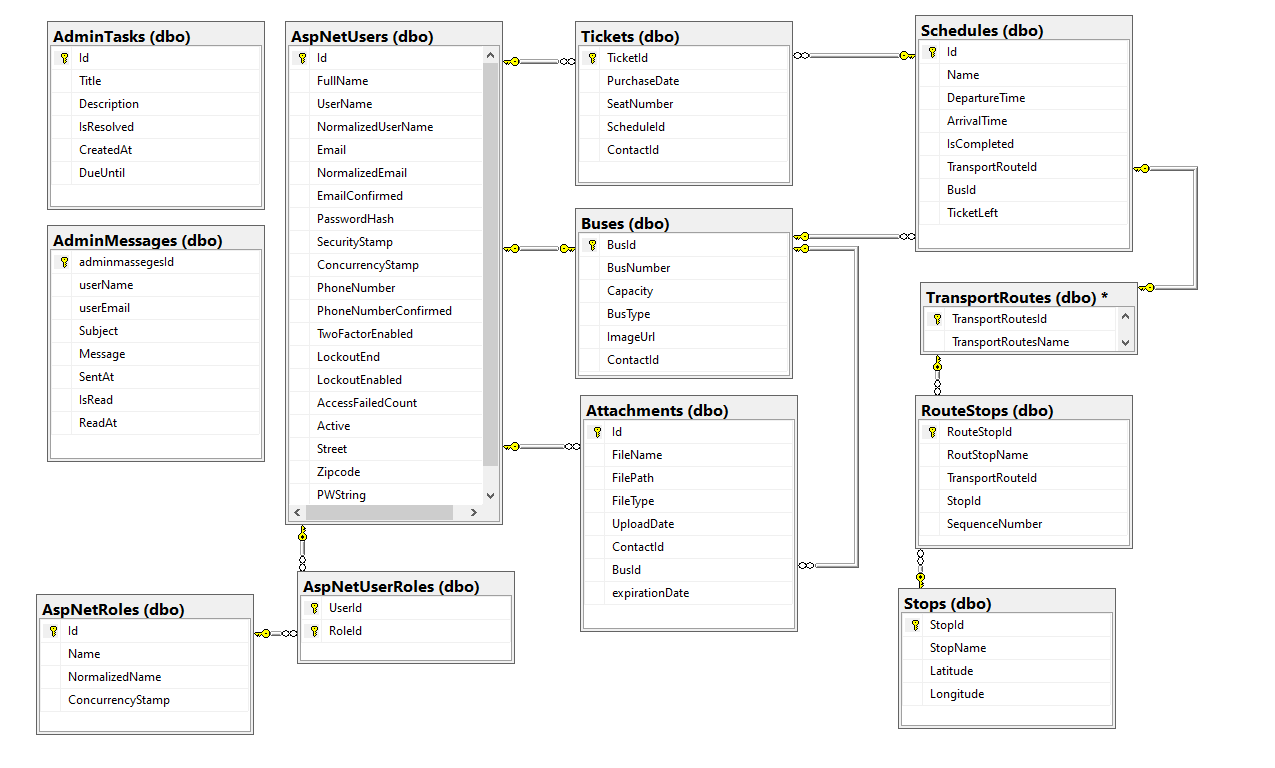
\includegraphics[width=1\textwidth]{Szakdolgozat/Mellekletek/ERfinal.PNG}
    

    \caption{Az adatbázis entitás-kapcsolat (E-K) diagramja}
    \label{fig:er-diagram}
\end{figure}

A \ref{fig:er-diagram}. ábrán látható az adatbázis logikai struktúrája.


\subsection{Felhasználói felület}

\indent A webalkalmazás felhasználói felületének kialakítása során elsődleges szempont volt az átláthatóság, a reszponzivitás, valamint a felhasználóbarát működés. A rendszer minden látogató számára egységes struktúrát biztosít, azonban a megjelenített tartalom és a hozzáférhető funkciók dinamikusan változnak a bejelentkezési állapot és a felhasználói szerepkör függvényében. A felület úgy került kialakításra, hogy mind a regisztrált utasok, mind az adminisztrátori jogosultsággal rendelkező felhasználók számára a szerepkörükkel releváns tartalom jelenjen meg.

\subsubsection{Főoldal}

\indent A kezdőlap minden látogató számára elérhető, és egy jól strukturált navigációs sávval segíti az alkalmazás fő funkcióinak gyors elérését. A menüsorban az alábbi pontok találhatók meg: \texttt{Stations}, \texttt{Routes}, \texttt{Schedules}, \texttt{MyTickets}, valamint a \texttt{Contact Us}. A jobb felső sarokban megjelenő opciók a látogató aktuális státuszától függenek. Be nem jelentkezett állapotban a \texttt{Login} és \texttt{Register} lehetőségek állnak rendelkezésre, míg bejelentkezett felhasználók esetében a \texttt{Profile} és a \texttt{Logout} gombok válnak láthatóvá. Amennyiben a bejelentkezett felhasználó adminisztrátori jogosultságokkal rendelkezik, egy további \texttt{Adminisztráció} legördülő menü is elérhetővé válik, amely az adminisztrációs funkciókhoz biztosít közvetlen hozzáférést.

\paragraph{Felhasználói nézet (utas szerepkör)}

\indent A rendszer általános felhasználói, azaz az utasok számára kialakított nézet célja, hogy a közlekedési szolgáltatások gyorsan és intuitív módon elérhetők legyenek. A kezdőoldalon keresztül megtekinthetők a vállalat által karbantartott megállók, amelyek földrajzi és logikai elhelyezkedésük alapján rendszerezettek. Az útvonalak menüpont segítségével a felhasználók megismerhetik az elérhető közlekedési útvonalakat, valamint az egyes útvonalakon szereplő megállókat is.

\indent A menetrendek áttekintése szintén kiemelt szerepet kap: az indulási időpontok, a járatokhoz tartozó útvonalak és a járművek együttesen jelennek meg, támogatva a tervezhető és hatékony utazást. A felhasználók számára elérhető a jegyvásárlási lehetőség is, amelyet vizuálisan kiemelt gomb segít megtalálni. A már megvásárolt jegyek a \texttt{MyTickets} szekcióban kerülnek listázásra, ahol a felhasználó saját jegyeit tekintheti át, függetlenül attól, hogy azok aktív vagy már lejárt foglalások. Ezen kívül a \texttt{Contact Us} menüpont egy kapcsolatfelvételi űrlapot biztosít, amelyen keresztül az adminisztráció számára üzenet küldhető, például észrevételek vagy kérdések esetén.

\indent Az egyszerű navigációs élmény részeként a jobb felső sarokban található profilmenü lehetőséget ad a személyes adatok megtekintésére és szerkesztésére. Ezáltal a felhasználók bármikor módosíthatják profiladataikat, illetve kijelentkezhetnek a rendszerből.

\paragraph{Adminisztrátori nézet}

\indent Az adminisztrátorok számára elérhető nézet jelentősen kibővített funkcionalitással rendelkezik. A bejelentkezést követően egy speciális \texttt{Adminisztráció} nevű legördülő menüpont válik aktívvá, amely az alkalmazás háttérrendszeréhez biztosít hozzáférést. Ennek segítségével az adminisztrátorok jogosultak új buszmegállók létrehozására, a meglévő megállók módosítására vagy törlésére. Az útvonalak karbantartása során lehetőség van új útvonalak definiálására, illetve a meglévők struktúrájának frissítésére.

\indent A menetrendek kezelése is része az adminisztrációs felületnek: az indulási időpontokhoz kapcsolódó adatok, valamint a jármű-hozzárendelések módosíthatók. A járműpark menedzselése során az autóbuszok nyilvántartása, adatszerkesztése és bővítése valósítható meg. Az adminisztrátorok hozzáférnek minden felhasználói jegyhez, így átfogó képet kapnak az utazási forgalomról.

\indent A rendszer lehetőséget biztosít a regisztrált felhasználók adatainak kezelésére is, beleértve az egyéni kapcsolattartási információkat és szerepköröket. A \texttt{ToDoList} funkció segítségével az adminisztrátorok belső feladatokat követhetnek nyomon. A beérkező felhasználói üzenetek külön felületen keresztül érhetők el, ahol válaszadásra is van lehetőség.

\indent További fontos adminisztratív funkció a szerepkörök kezelése: az adminisztrátorok új szerepköröket definiálhatnak, illetve módosíthatják a meglévőeket (pl. utas, alkalmazott, adminisztrátor), ezzel szabályozva a hozzáférési jogosultságokat az alkalmazás különböző moduljaihoz.

\indent Míg az utas szerepkörrel rendelkező felhasználók jellemzően csak megtekintési jogosultsággal rendelkeznek, addig az adminisztrátorok számára minden entitáson elérhetővé válik a teljes CRUD-funkcionalitás (Create, Read, Update, Delete). Ez a szerepköralapú jogosultságkezelés biztosítja, hogy a rendszer minden felhasználó számára csak az általa engedélyezett műveletek legyenek elérhetők, miközben a felület egységes marad.
\begin{figure}[H]
    \centering
    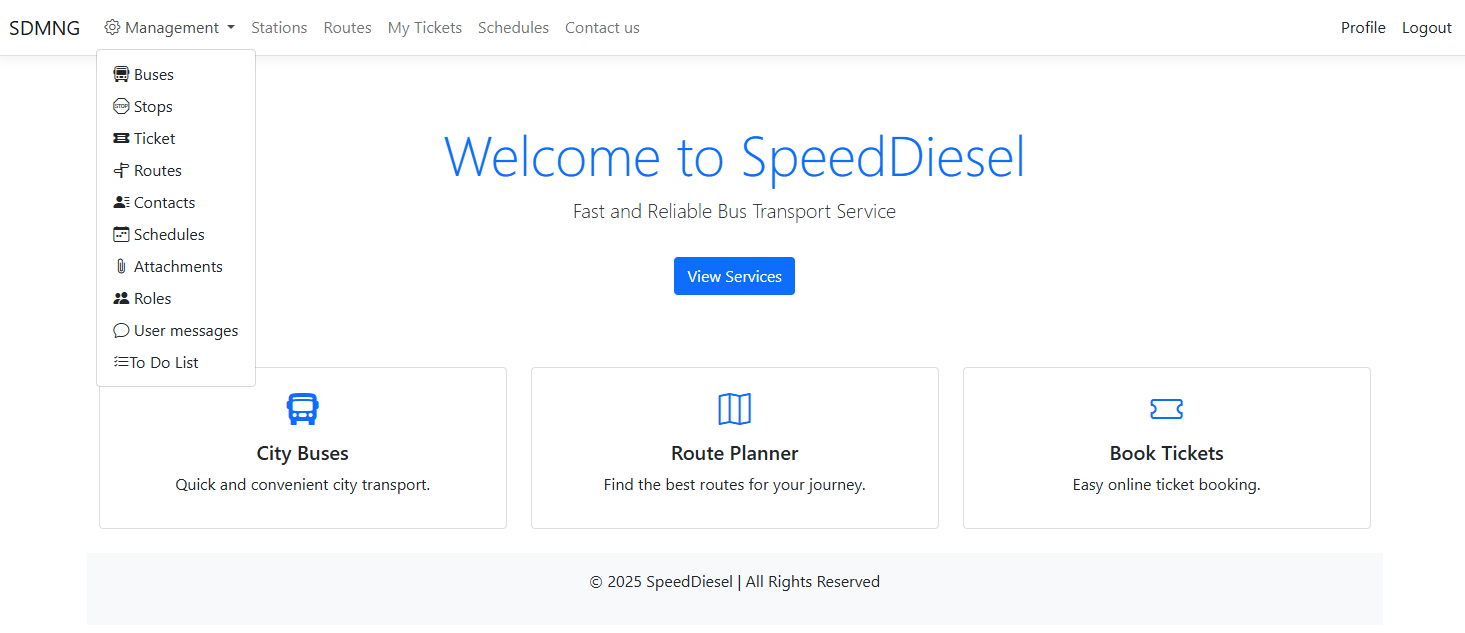
\includegraphics[width=1\textwidth]{Szakdolgozat/Mellekletek/fooldal.PNG}
    \caption{A rendszer főoldala adminisztrátori bejelentkezés után, látható \texttt{Management} menüvel}
    \label{fig:admin-home}
\end{figure}

A \ref{fig:admin-home}. ábra a rendszer főoldalát mutatja be olyan nézetben, amely adminisztrátori jogosultságokkal rendelkező felhasználó számára érhető el. A főmenüsorban jól megfigyelhető a \texttt{Management} lenyíló menüpont, amely kizárólag adminisztrátorok számára jelenik meg. Ezen keresztül elérhetők az adminisztratív funkciók, például megállók, útvonalak, menetrendek és felhasználók kezelése.

\subsubsection{Bejelentkezési oldal (Login)}

A bejelentkezési felületen a felhasználó e-mail címe és jelszava megadásával tud belépni a rendszerbe. Emellett lehetőség van jelszóemlékeztető kérésére is, egy opcionális „Elfelejtett jelszó” linken keresztül. Sikeres bejelentkezést követően a rendszer automatikusan visszairányítja a felhasználót a főoldalra.

\subsubsection{Regisztrációs oldal (Register)}

A regisztrációs oldalon a felhasználó egy egyszerű űrlap kitöltésével hozhat létre új fiókot. Az űrlap a felhasználó nevét, e-mail címét, jelszavát, valamint a szándék megerősítését igényli. A regisztrációt követően a rendszer automatikusan átirányíthatja a bejelentkezési oldalra.

\subsubsection{Stations oldal}

A \texttt{Stations} oldal a rendszer összes regisztrált megállóját listázza. A felhasználói élmény és funkciók a felhasználó szerepkörétől függően változnak, ezért az oldal két különálló nézettel rendelkezik: egy publikus, információs nézettel az utasok számára, valamint egy bővített kezelőfelülettel az adminisztrátorok részére.

\paragraph{Felhasználói nézet (publikus elérés)}

Amennyiben az oldal a főmenüből kerül megnyitásra, a rendszer a látogatók és bejelentkezett utasok számára elérhető változatot jeleníti meg. Ebben a nézetben egy táblázat jelenik meg, amely az összes megállót felsorolja, az alábbi oszlopokkal: \texttt{StopName}, \texttt{Latitude}, \texttt{Longitude}, valamint \texttt{Actions}. Az \texttt{Actions} oszlopban kizárólag egy \texttt{Details} gomb található, amely lehetőséget biztosít az adott megálló részletes adatainak megtekintésére.

A \texttt{Details} gombra kattintva a felhasználó egy különálló nézetre navigál, ahol az adott megálló részletes információi jelennek meg. A felületen szerepel a megálló neve, a földrajzi koordinátái (szélességi és hosszúsági adatok), valamint egy térképes megjelenítés, amely vizuálisan is elhelyezi a megállót a térképen, egy ponttal jelölve annak pontos helyzetét. Ez a nézet teljes mértékben információközlő jellegű, módosítási vagy törlési lehetőséget nem kínál.

\paragraph{Adminisztrátori nézet}

Ha az oldalt az adminisztrációs menüpont \texttt{Stops} almenüjén keresztül nyitjuk meg, a rendszer egy másik nézetet jelenít meg, amely kifejezetten az adminisztrátori szerepkörrel rendelkező felhasználók számára lett kialakítva. Ez a felület nemcsak az adatok megtekintését teszi lehetővé, hanem adminisztratív műveletek végrehajtását is engedélyezi. A táblázatos elrendezés ebben a nézetben megegyezik a publikus nézet szerkezetével — ugyanazok az oszlopok jelennek meg (\texttt{StopName}, \texttt{Latitude}, \texttt{Longitude}, \texttt{Actions}) —, azonban az \texttt{Actions} oszlopban több lehetőség is elérhető. A \texttt{Details} gomb mellett megjelennek a \texttt{Edit} és \texttt{Delete} gombok is, amelyekkel a megálló adatainak szerkesztése, illetve törlése valósítható meg.

Ezen kívül az adminisztrátorok számára elérhető egy \texttt{Create New Stop} gomb is, amely új megállók hozzáadására szolgál. Fontos kiemelni, hogy az adminisztrátorok hozzáférnek a publikus részletező nézethez is, így ők is megtekinthetik ugyanazt az információgazdag, térképes megjelenítést, amely a látogatók és utasok számára is elérhető. Ez lehetővé teszi számukra, hogy a szerkesztési vagy törlési műveletek előtt pontosan ellenőrizzék a megállók földrajzi elhelyezkedését.

Mindkét nézet ugyanazt az adatstruktúrát használja a megállók megjelenítésére, azonban a funkcionális lehetőségek jelentősen eltérnek a felhasználói szerepkörtől függően. A kialakítás célja, hogy egy átlátható, könnyen kezelhető felületet biztosítson mind az információra kíváncsi utasok, mind pedig az adminisztratív műveleteket végző rendszerkezelők számára.

\begin{figure}[H]
    \centering
    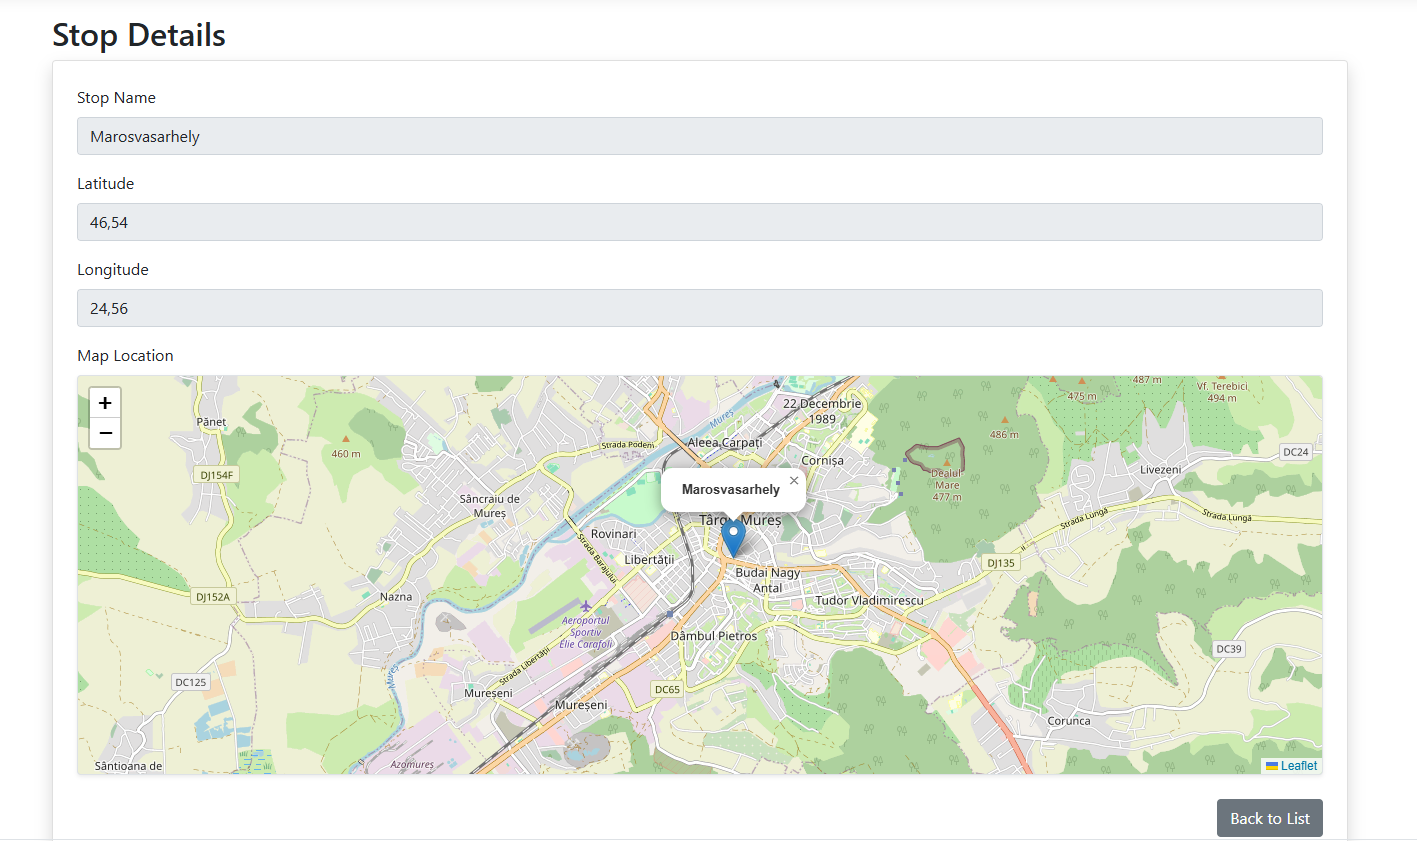
\includegraphics[width=1\textwidth]{Szakdolgozat/Mellekletek/StopDetail.PNG}
    \caption{Megálló részletes adatlapja felhasználói nézetben, térképes megjelenítéssel}
    \label{fig:stop-detail-user}
\end{figure}

A \ref{fig:stop-detail-user}. ábra egy megálló részletes adatlapját szemlélteti olyan formában, ahogyan azt egy általános felhasználó látja, aki a főmenüből navigált erre az oldalra.

Fontos megjegyezni, hogy adminisztrátori jogosultság esetén az ugyanilyen részletes nézet tartalmilag hasonló, azonban a térképes megjelenítés hiányzik belőle. Mivel az adminisztrátorok a megállók kezelését más, célzott nézetekből végzik (pl. a kezelőfelület táblázatos listájából kiindulva), a részletes oldal csupán kiegészítő információként szolgál számukra.


\subsubsection{Routes oldal}

A \texttt{Routes} oldalon a rendszer az adatbázisban szereplő összes elérhető útvonalat listázza. Ennek a felhasználói felület azért szükséges, hogy a látogatók és regisztrált utasok könnyen áttekintést kapjanak az egyes útvonalakról, míg az adminisztrátorok számára részletes kezelési lehetőségeket is biztosít.

\paragraph{Felhasználói nézet (publikus elérés)}

Amennyiben az oldalt a főmenüből érjük el, a rendszer a látogatók és bejelentkezett utasok számára elérhető nézetet jeleníti meg. A megjelenő táblázat az alábbi oszlopokat tartalmazza: \texttt{Name} (az útvonal megnevezése), \texttt{Stops} (egész számként jelölve, hogy hány megállót tartalmaz az adott útvonal), valamint az \texttt{Actions} oszlop, amely egyetlen \texttt{Details} gombot tartalmaz. A felhasználók ezen keresztül tekinthetik meg az adott útvonal részletes információit.

A \texttt{Details} gombra kattintva a felhasználó egy részletes nézethez jut, amely az adott útvonalra vonatkozó információkat jeleníti meg. Az oldal felső részén látható az útvonal neve, alatta pedig egy térkép, amely vizuálisan ábrázolja a megállókat összekötő vonal mentén az útvonalat. A térképet követően egy táblázat jelenik meg, amely sorolja a megállók sorrendjét (\texttt{Index}), nevét, földrajzi szélességi és hosszúsági koordinátáit. Ez a felület kizárólag az információk megtekintésére szolgál, szerkesztési vagy módosítási lehetőséget nem kínál.

\paragraph{Adminisztrátori nézet}

Amennyiben az oldalt az \texttt{Adminisztráció} menüpont \texttt{Routes} opcióján keresztül nyitjuk meg, a rendszer egy adminisztrátori funkciókkal bővített nézetet tölt be. A megjelenő táblázat szerkezete megegyezik a publikus változattal (\texttt{Name}, \texttt{Stops}, \texttt{Actions}), azonban az \texttt{Actions} oszlopban nemcsak a \texttt{Details}, hanem az \texttt{Edit} és \texttt{Delete} gombok is elérhetők, lehetővé téve az útvonalak módosítását vagy törlését. A táblázat felett egy \texttt{Create New Route} gomb is található, amely új útvonalak létrehozására szolgál.

Az adminisztrátor által megnyitott részletes nézet az útvonalhoz rendelt megállókat egy belső táblázatban sorolja fel. Itt az egyes sorok a megállók sorrendi sorszámát, nevét, valamint földrajzi koordinátáit tartalmazzák. A táblázat ezen felül egy \texttt{Actions} oszlopot is tartalmaz, ahol minden megálló mellett elérhető egy \texttt{Delete} gomb. Ennek segítségével az adott megálló eltávolítható az útvonalból, anélkül hogy maga a megálló törlődne az adatbázisból. A táblázat alatt egy lenyíló mező és egy \texttt{Add Stop to Route} gomb található, amelyek új megálló hozzárendelését teszik lehetővé az adott útvonalhoz.

\begin{figure}[H]
    \centering
    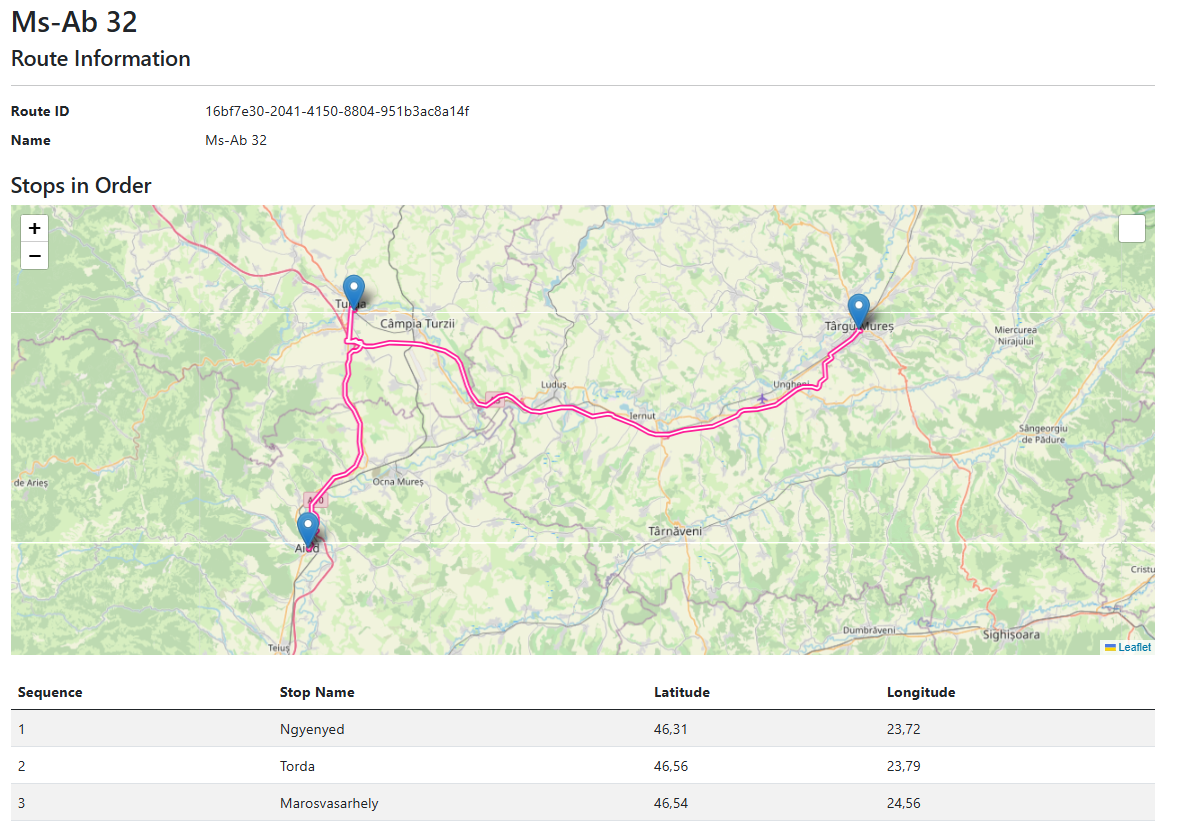
\includegraphics[width=1\textwidth]{Szakdolgozat/Mellekletek/RoutesDetail.PNG}
    \caption{Útvonal részletes adatlapja felhasználói nézetben, térképes megjelenítéssel}
    \label{fig:route-detail-user}
\end{figure}

A \ref{fig:route-detail-user}. ábra egy útvonal részletes adatlapját mutatja be, ahogyan azt egy bejelentkezett felhasználó látja, aki a főmenüből navigált az adott útvonal információihoz. Az adott példában a Nagyenyed–Torda–Marosvásárhely útvonal vizualizációja figyelhető meg.


\subsubsection{Schedules oldal}

A \texttt{Schedules} oldalon a felhasználók a menetrendeket böngészhetik, amelyeket dátum, időpont, útvonal és a közlekedő busz szerint csoportosít a rendszer. Amennyiben az adott járaton van szabad ülőhely, lehetőség van jegyvásárlásra is. Az adminisztrátorok teljes körű menetrendkezelést végezhetnek: új menetrendeket adhatnak hozzá, szerkeszthetik vagy törölhetik a meglévőket, valamint hozzárendelhetik a kiválasztott útvonalakat és autóbuszokat.

\subsubsection{MyTicket oldal}

A \texttt{MyTicket} oldal célja a rendszerben rögzített jegyvásárlások megjelenítése és áttekintése. Az oldal két különböző nézetet biztosít a felhasználói szerepkör függvényében: egyet az általános felhasználók (utasok), egy másikat pedig az adminisztrátorok számára. 

\paragraph{Felhasználói nézet (utasok részére)}

Amennyiben egy bejelentkezett felhasználó navigál a \texttt{MyTicket} oldalra, a rendszer kizárólag az adott személyhez tartozó jegyeket jeleníti meg. A felületen egy táblázat látható, amely a következő oszlopokat tartalmazza: \texttt{TicketId}, \texttt{PurchaseDate}, \texttt{SeatNumber}, \texttt{User} (automatikusan az aktuális felhasználó), \texttt{Schedule}, valamint az \texttt{Actions} oszlop. Az \texttt{Actions} oszlopban egyetlen műveletgomb kap helyet: a \texttt{Details}, amely az adott jegy részletes adatlapjára irányít.

A \texttt{Details} nézetben a felhasználó bővebb információkat kap a jegyhez tartozó menetrendről, beleértve az indulási és érkezési állomásokat, a járat buszának rendszámát, illetve megjelenik egy interaktív térkép is, amely az utazás útvonalát vizuálisan ábrázolja. Ez az ábra segíti az utasokat az útvonal pontos áttekintésében, és kiegészíti az egyéb szöveges információkat.

\paragraph{Adminisztrátori nézet}

Az adminisztrátorok számára a \texttt{Tickets} oldal a \texttt{Management} menüponton keresztül érhető el, ahol az összes, a rendszerben rögzített jegy megjelenik, függetlenül attól, hogy mely felhasználó vásárolta meg őket. Az itt található táblázat szerkezete megegyezik a felhasználói nézettel, azzal a különbséggel, hogy a \texttt{User} oszlopban minden jegyhez tartozó felhasználó kiléte is feltüntetésre kerül. Ez lehetővé teszi az adminisztrátorok számára a jegyek teljes körű nyomon követését és kezelését.

A táblázat \texttt{Actions} oszlopában három funkciógomb található: \texttt{Details}, \texttt{Edit} és \texttt{Delete}. A \texttt{Details} gombbal megnyitható a jegy részletes adatlapja, ahol bővebb információk jelennek meg az adott utazásról, míg az \texttt{Edit} és \texttt{Delete} gombokkal az adminisztrátor módosíthatja vagy törölheti az adott jegyet. Ezzel biztosított a teljes adminisztratív kontroll az összes jegy felett.

Az admin nézet részletes felülete struktúrájában hasonló a felhasználói nézethez, azonban itt nem szerepel a térképes útvonalmegjelenítés. A hangsúly inkább az adatok rendszerezett és pontos bemutatásán van: ide tartoznak az indulási és érkezési megállók, a menetrend adatai, a járat azonosítója és a kapcsolódó felhasználói információk.

Ez az oldal különösen informatív és részletes, összevetve más, jelenleg használatban lévő közlekedési rendszerekkel. Míg sok hasonló alkalmazásban a jegykezelés csupán alapinformációkra szorítkozik, itt az adminisztrátorok számára biztosított minden szükséges funkció a hatékony kezeléshez és ellenőrzéshez.



\subsubsection{Contact Us oldal}

A \texttt{Contact Us} oldal elsődleges célja, hogy lehetőséget biztosítson a látogatók számára az adminisztrátorral való közvetlen kapcsolatfelvételre. Ez az oldal nyilvánosan elérhető, így használatához nincs szükség bejelentkezésre, ami különösen fontos szempont volt a tervezés során. A kapcsolatfelvételi felület egy egyszerűen kezelhető űrlapot tartalmaz, amely négy mezőből áll: a feladó neve (\texttt{Name}), e-mail címe (\texttt{Email}), az üzenet tárgya (\texttt{Subject}) és maga az üzenet tartalma (\texttt{Message}).

A felhasználó az űrlap kitöltését követően a \texttt{Send} gomb segítségével tudja elküldeni az üzenetet. A rendszer a beküldött adatokat automatikusan elmenti az adatbázis megfelelő táblájába, így az adminisztrátorok később visszakereshetik azokat. Emellett a rendszer e-mail értesítést is küld az adminisztrátori címre, amely tartalmazza a megadott adatokat, lehetővé téve a gyors reagálást.

Fontos megjegyezni, hogy ez az oldal kizárólag a felhasználói felületen érhető el, és nem része az admin menüpontoknak. Az alkalmazás ezzel a funkcióval lehetőséget biztosít arra, hogy a látogatók közvetlenül visszajelzést küldjenek, kérdéseket tegyenek fel vagy hibát jelentsenek, így támogatva a folyamatos fejlesztést és felhasználói elégedettséget.

\subsubsection{Adminisztrációs oldalak}

A rendszer adminisztrátori jogosultságokkal rendelkező felhasználói számára külön menüpontok érhetők el a felhasználói felület felső navigációs sávjában található \texttt{Management} legördülő menüben. Ezek a funkciók kizárólag az adminisztrátorok számára hozzáférhetők, céljuk a rendszer különböző erőforrásainak és entitásainak karbantartása és felügyelete.

A menüpontok közül a \texttt{Contacts} oldal tartalmazza a rendszerbe regisztrált összes felhasználót – ideértve az adminisztrátorokat, munkatársakat és általános felhasználókat egyaránt. Az oldal megnyitásakor egy táblázatos nézet fogadja a felhasználót, amely a következő adatmezőket jeleníti meg: \texttt{FullName}, \texttt{Email}, \texttt{Street}, \texttt{Zipcode}, \texttt{Active}, \texttt{Bus}, valamint az \texttt{Actions} oszlop. Az \texttt{Actions} oszlopban három gomb kapott helyet, amelyek lehetővé teszik a kiválasztott felhasználó adatainak részletes megtekintését, szerkesztését vagy törlését (\texttt{Detail}, \texttt{Edit}, \texttt{Delete}). A táblázat alatt egy külön gomb is található, amely új felhasználó manuális hozzáadását teszi lehetővé, ezáltal bővítve az adminisztrátor lehetőségeit a rendszer kézi karbantartása során.

A három elérhető műveleti gomb mindegyike hasonló szerkezetű oldalra navigál, azonban az adott funkciónak megfelelően eltérő célokat szolgál. A részletes megtekintés során az adminisztrátor az adott felhasználó összes adatát áttekintheti egy jól strukturált nézetben, míg a szerkesztés során ezen adatok módosítására is lehetőség nyílik. A törlés funkció egy deaktivációs müvelet legyen, ne töröljünk felhasználókat, csak ideiglenesen legyenek inaktívak.

Minden nézet tartalmazza azokat az információkat, amelyek az adminisztrációs táblázatban is szerepelnek (név, e-mail, cím stb.), azonban ezeken túl két további mező is megjelenik: a felhasználóhoz rendelt szerepkör (\texttt{Role}), valamint az adott felhasználóhoz társított autóbusz megléte vagy hiánya. Ez utóbbi információ különösen fontos a buszvezetői szerepköröknél, mivel ezek a jogosultságok gyakran kapcsolódnak konkrét járművekhez. Az adminisztrátor így átfogó képet kap a felhasználók státuszáról, jogosultságairól és az esetleges operatív hozzárendelésekről is.

A szerkesztési nézet (\texttt{Edit}) további fontos funkcióval is bővül. Ebben a nézetben ugyanis lehetőség nyílik a kiválasztott felhasználó szerepkörének módosítására egy legördülő menü segítségével. Ezáltal az admin dönthet arról, hogy az adott felhasználó egyszerű felhasználó, adminisztrátor vagy más speciális szerepkört töltsön be a rendszerben. Hasonlóképpen, a rendszer lehetőséget biztosít arra is, hogy az admin egy konkrét autóbuszt rendeljen hozzá a kiválasztott felhasználóhoz, amennyiben az adott szerepkör ezt megengedi. Mindkét funkció csak az admin jogosultsággal rendelkező személyek számára érhető el, az általános felhasználók nem tudják ezeket az attribútumokat módosítani, ezáltal garantálva a rendszer adatainak integritását és a jogosultságkezelés biztonságát.

A \texttt{Buses} oldal az adminisztrátorok számára elérhető felület, amely lehetővé teszi a rendszerben nyilvántartott autóbuszok kezelését. Az oldalra lépve egy áttekinthető táblázat fogadja a felhasználót, amely az egyes járművek legfontosabb adatait sorolja fel: \texttt{BusNumber} (rendszám), \texttt{Capacity} (férőhelyek száma), \texttt{BusType} (járműtípus), \texttt{ImageUrl} (a járműhöz tartozó kép elérési útvonala), valamint az \texttt{Actions} oszlop, ahol a megszokott \texttt{Detail}, \texttt{Edit} és \texttt{Delete} gombok segítségével hajthatók végre a különféle műveletek. Ezek az akciók minden esetben a megfelelő, funkcionálisan elkülönített nézetekre vezetnek, ahol a járműadatok megtekintése, módosítása vagy törlése történik.

A táblázat alján elhelyezett gomb egy új autóbusz hozzáadására szolgál, és a \texttt{Create Bus} oldalra navigál, ahol a felhasználónak lehetősége van megadni az új jármű alapadatait: \texttt{BusNumber}, \texttt{Capacity}, valamint a \texttt{BusType}. Ezen kívül egy speciális kiválasztó mező is elérhető, amelynek segítségével hozzárendelhető egy sofőr az adott buszhoz – ez azonban kizárólag admin jogosultság esetén látható és használható. A kiválasztás csak a rendszerben szereplő, megfelelő szerepkörrel rendelkező felhasználók közül történhet.

Az egyes autóbuszokra kattintva elérhető \texttt{Detail} nézet szintén az említett adatokat jeleníti meg, kiegészítve az adott járműhöz rendelt sofőr nevével is. Ez a megjelenítés nemcsak az adminisztratív nyilvántartást könnyíti meg, hanem átláthatóvá teszi a felelősségi viszonyokat is, amely különösen hasznos lehet nagyobb flotta kezelésekor. Ezen kívül a részletes oldalon található egy \texttt{Add Attachment} gomb is, amely egy külön felületre irányít, ahol az adminisztrátor fájlokat – például műszaki dokumentációt vagy engedélyeket – csatolhat a járműhöz egy kiválasztómező segítségével. Ez a kiegészítő funkció lehetővé teszi a dokumentumkezelés központosítását és rendszerezését a járművekhez kapcsolódóan.

Az \texttt{Attachments} oldal az adminisztrátorok számára biztosít hozzáférést a rendszerben tárolt valamennyi melléklethez. Az oldalon egy áttekintő táblázat található, amelyben minden fájlhoz kapcsolódó alapinformáció megjelenik. A felsorolt adatok a következők: \texttt{FileName} (a fájl neve), \texttt{FileType} (típusa), \texttt{UploadDate} (feltöltés dátuma), \texttt{ExpirationDate} (lejárati dátuma), \texttt{FullName} (a melléklethez kapcsolt felhasználó neve), valamint \texttt{BusNumber} (az érintett jármű rendszáma). A \texttt{UploadDate} mindig a tényleges feltöltési időpontot mutatja, míg az \texttt{ExpirationDate} automatikusan egy évvel későbbre kerül beállításra.

A rendszer biztosítja, hogy minden melléklet vagy egy felhasználóhoz (\texttt{Contact}), vagy egy autóbuszhoz (\texttt{Bus}) legyen hozzárendelve – egyszerre azonban csak az egyikhez. Abban az esetben, ha az egyik kapcsolat nem kerül megadásra, az adott mező \texttt{NA} (Not Assigned) értéket kap a táblázatban, ezzel jelezve a hiányzó kapcsolatot.

A táblázat utolsó oszlopában találhatóak az adminisztrációs műveleteket biztosító gombok, nevezetesen a \texttt{Detail}, \texttt{Edit} és \texttt{Delete} opciók, amelyek lehetőséget nyújtanak az adott melléklet adatainak megtekintésére, módosítására vagy törlésére. Ezek a funkciók az admin felhasználók részére elérhetőek, és minden esetben biztosítják a csatolmányok pontos nyilvántartását.

Új melléklet hozzáadására ezen az oldalon nincs lehetőség, mivel a feltöltési művelet kizárólag az érintett felhasználó vagy autóbusz részletes adatlapjáról indítható. Az ott elhelyezett \texttt{Add Attachment} gomb segítségével lehet kiválasztani és csatolni a kívánt dokumentumot, amely ezáltal automatikusan a megfelelő entitáshoz kerül kapcsolásra. Ez a struktúra lehetővé teszi az adatok pontos szervezését és visszakereshetőségét, miközben kizárólag az adminisztrátorok számára biztosítja a hozzáférést és módosítási jogosultságot.

Az \texttt{User Messages} oldal az adminisztrátorok számára készült, és a felhasználóktól érkező kapcsolatfelvételi üzenetek kezelésére szolgál. Ez az oldal a \texttt{Management} menüpont alól érhető el, és tartalmazza az összes olyan bejegyzést, amely a \texttt{Contact Us} űrlap kitöltésével került rögzítésre a rendszerben. A megjelenített táblázat minden üzenetet listáz, függetlenül attól, hogy azokat már megtekintették-e vagy sem.

A táblázat oszlopai a következő információkat jelenítik meg: \texttt{UserName} (a feladó neve), \texttt{UserEmail} (az e-mail címe), \texttt{Subject} (az üzenet tárgya), \texttt{SentAt} (küldés időpontja), valamint az \texttt{IsRead} mező, amely azt jelzi, hogy az adott üzenetet az admin már megnyitotta-e. A rendszer automatikusan nyomon követi az üzenetek megtekintését: amint az adminisztrátor rákattint a \texttt{Detail} gombra és megnyitja az adott bejegyzést, az \texttt{IsRead} értéke automatikusan \texttt{true}-ra változik, így a későbbiekben is egyértelműen nyomon követhető, mely üzenetek lettek már feldolgozva.

Az \texttt{Actions} oszlop egyetlen gombot tartalmaz, amely a részletek megtekintésére szolgál. A megnyitott nézetben az admin elolvashatja a felhasználó által küldött teljes üzenetet. A rendszer nem biztosít lehetőséget ezen üzenetek szerkesztésére vagy törlésére, hiszen ezek kizárólag tájékoztatási célból kerülnek be az adatbázisba.

Fontos kiemelni, hogy ezen az oldalon nem áll rendelkezésre új üzenet manuális hozzáadására szolgáló funkció, mivel az összes bejegyzés kizárólag a felhasználói űrlap kitöltésével jöhet létre. Az oldal célja a felhasználói visszajelzések átlátható, hatékony kezelése és archiválása az adminisztráció számára.

A \texttt{ToDoList} menüpont az adminisztrátorok számára elérhető, és a rendszerben végzendő feladatok kezelését teszi lehetővé. Ez az oldal interaktívabb megközelítést alkalmaz, mint a többi adminisztrációs felület, mivel nem csupán adatokat jelenít meg, hanem lehetőséget biztosít az egyéni feladatok nyomon követésére és kezelésére is.

Az oldal betöltésekor egy áttekinthető táblázat jelenik meg, amely minden korábban létrehozott feladatot tartalmaz. A táblázat három fő oszlopból áll: \texttt{Title} (a feladat címe), \texttt{Due} (a határidő), valamint az \texttt{Actions} oszlop, amely két műveleti gombot tartalmaz. Ezek közül a \texttt{Detail} gomb a feladat részleteit jeleníti meg, míg az \texttt{Edit} gomb közvetlenül a szerkesztőfelületre navigál.

A részletes nézet szintén tartalmaz egy \texttt{Szerkesztés} gombot, amely ugyanarra az \texttt{Edit} oldalra visz tovább. Mind a részletes nézetben, mind pedig a szerkesztőfelületen a feladat alábbi mezői jelennek meg: a cím, a határidő és egy jelölőnégyzet, amellyel a feladat státusza állítható be – ez azt mutatja, hogy a feladat elvégzése megtörtént-e. Ennek a mezőnek a bejelölésével a feladat „készre jelenthető”.

A feladatok vizuálisan is jól elkülöníthetők az állapotuk alapján: a már teljesített feladatokat a rendszer zöld háttérrel jeleníti meg, míg a még el nem végzetteket fehéren emeli ki. Ez a színkódolás segíti az adminokat abban, hogy gyorsan átlássák az aktuális teendőket, és azonnal be tudják azonosítani a sürgős feladatokat.


\begin{figure}[H]
\centering
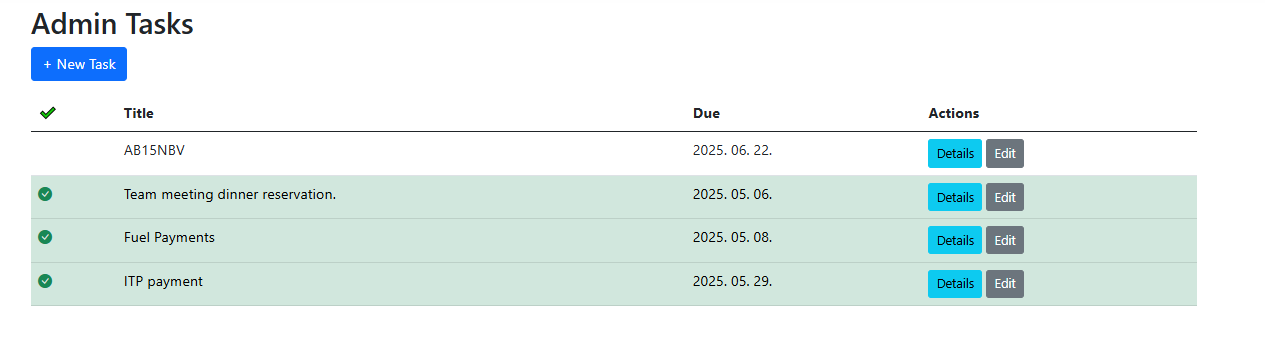
\includegraphics[width=1\textwidth]{Szakdolgozat/Mellekletek/admintasks.PNG}
\caption{Adminisztrátori feladatok listája látható }
\label{fig:todo-admintask}
\end{figure}

A \ref{fig:todo-admintask}. ábra az adminisztrátorok számára elérhető \texttt{ToDoList} oldal listanézetét szemlélteti, ahol az aktuális feladatok áttekinthető formában jelennek meg.

\newpage
\section{Megvalósítás}

Ebben a fejezetben részletesen bemutatásra kerül a rendszer megvalósítása, a projekt kezdeti létrehozásától kezdve a mappa- és fájlstruktúra leírásán át a legfontosabb funkciók implementációjáig. A cél egy átláthatóan felépített alkalmazás létrehozása, amely mind a felhasználói, mind az adminisztratív felületen stabil és könnyen karbantartható működést biztosít.

\subsection{A projekt létrehozása és környezet beállítása}

A fejlesztés Microsoft Visual Studio 2022 környezetben valósult meg, a .NET 8.0 keretrendszerre építve. A projekt típusa \textit{ASP.NET Core MVC Web Application}, amely a model-view-controller (MVC) architektúra elveit követi, lehetővé téve az üzleti logika, a megjelenítés és az adatkezelés hatékony rendszerezését.

Az adatkezeléshez az Entity Framework Core komponenst használtam, a Code First megközelítés segítségével. Az Entity Framework Core egy modern ORM( Object-Relational Mapping) technológia a .NET alkalmazások számára, amely lehetővé teszi az adatbázis-műveletek magas szintű megvalósítását. Ennek köszönhetően a modellosztályok a programkódban lettek definiálva, majd migrációk létrehozásával az adatbázis-struktúra automatikusan generálódott. Ez a módszer rugalmasságot biztosít a fejlesztés során, és egyszerűsíti az adatbázis módosítását.

Az alkalmazás egy SQL Server Express alapú relációs adatbázist használ, amely helyi környezetben gyors, megbízható és könnyen konfigurálható megoldást biztosít a fejlesztéshez. Az adatbázis kezelése teljesen az Entity Framework migrációs rendszerére épül.

\subsection{A megvalósítás mappastruktúrája és fő komponensei}

A projekt létrehozása a Visual Studio 2022 fejlesztőkörnyezet és a .NET 8 keretrendszer segítségével valósult meg. Az így generált mappastruktúra jól rendszerezett és könnyen bővíthető, támogatja az átlátható fejlesztést, és megkönnyíti az egyes komponensek logikai szétválasztását.

A \texttt{Controllers} mappa azokat az osztályokat tartalmazza, amelyek a felhasználói interakciókat kezelik és az adatokat feldolgozzák a működési logika szerint. Ezek a vezérlők külön-külön foglalkoznak az egyes entitásokkal, például a menetrendekkel, jegyekkel vagy felhasználókkal, biztosítva az adatok és a nézetek közötti kapcsolatot.

A \texttt{Models} könyvtár tartalmazza azokat az osztályokat, amelyek az adatbázisban tárolt entitásokat képezik, például a \texttt{Ticket}, \texttt{Contact} vagy \texttt{Schedule} osztályokat. Ezek az osztályok felelősek az adatok szerkezetének és az entitások közötti kapcsolatok megvalósításáért. Tulajdonképpen ezek az osztályok képezik az adatbázis tábláinak mintáját.


\subsection{Adatmodell és adatbázis felépítése}

Miután a projektet létrehoztam, elsőként az alkalmazás alapját képező osztályokat, azaz a modelleket kellett létrehozni. Ezek az osztályok az adatbázisban tárolt adattáblákat írják le, és tartalmazzák a hozzájuk tartozó tulajdonságokat, valamint az egymással kialakított relációkat. Az előzetesen elkészített adatbázis-terv alapján hoztam létre az \texttt{AdminMessage}, \texttt{AdminTask}, \texttt{Attachment}, \texttt{Bus}, \texttt{Contact}, \texttt{RouteStop}, \texttt{Schedule}, \texttt{Stop}, \texttt{Ticket}, valamint \texttt{TransportRoute} osztályokat. Fontos kritérium volt, hogy az entitások közötti relációkat pontosan és figyelmesen implementáljuk. Itt az elsődleges kulcsok (Primary Key), illetve az idegen kulcsok (Foreign Key) helyes használatára kellett különös figyelmet fordítani.

\subsubsection{Contact osztály}
Az alkalmazás felhasználókezelését az ASP.NET Identity keretrendszerre építettem, amely beépített mechanizmusokat biztosít a hitelesítés, az engedélyezés és a szerepkörök kezelésének megvalósításához. A rendszer egyik alapkövét a \texttt{Contact} osztály képezi, amely az \texttt{IdentityUser} osztályból származik, így örökli annak minden alapvető tulajdonságát, például a felhasználónév, e-mail, jelszóhash és biztonsági token mezőket.

Ezt az alapstruktúrát a saját igényeim szerint bővítettem ki további tulajdonságokkal, mint például a felhasználó teljes neve (\texttt{FullName}), címe (\texttt{Street}, \texttt{Zipcode}), aktív státusza (\texttt{Active}), illetve a jelszó nyers formában történő ideiglenes tárolása (\texttt{PWString}). Útóbbit a könnyebb tesztelés és használat érdekében adtam hozzá. A modell a relációs adatbázisok világához igazodva navigációs kapcsolatokat is tartalmaz más entitásokkal, például a \texttt{Ticket} vagy \texttt{Attachment} osztályokkal.


\subsubsection{AppDbContext}
Ezen felül az \texttt{AppDbContext} lehetőséget biztosít az entitások viselkedésének testreszabására az \texttt{OnModelCreating} metódusban, ahol külön definiálhatjuk a kulcsokat, kapcsolatokat, korlátozásokat, valamint egyéb konfigurációkat. Különösen hasznos az úgynevezett "vízesés törlés" (cascade delete) viselkedés figyelembe vétele, amely során egy entitás törlése vízesésszerűen magával vonhatja más kapcsolódó entitások törlését is. Az \texttt{OnModelCreating} metódus lehetőséget biztosít ennek felügyelésére, ezáltal elkerülve az adatvesztést okozó nem kívánt láncfolyamatokat.

\begin{figure}[H]
\centering
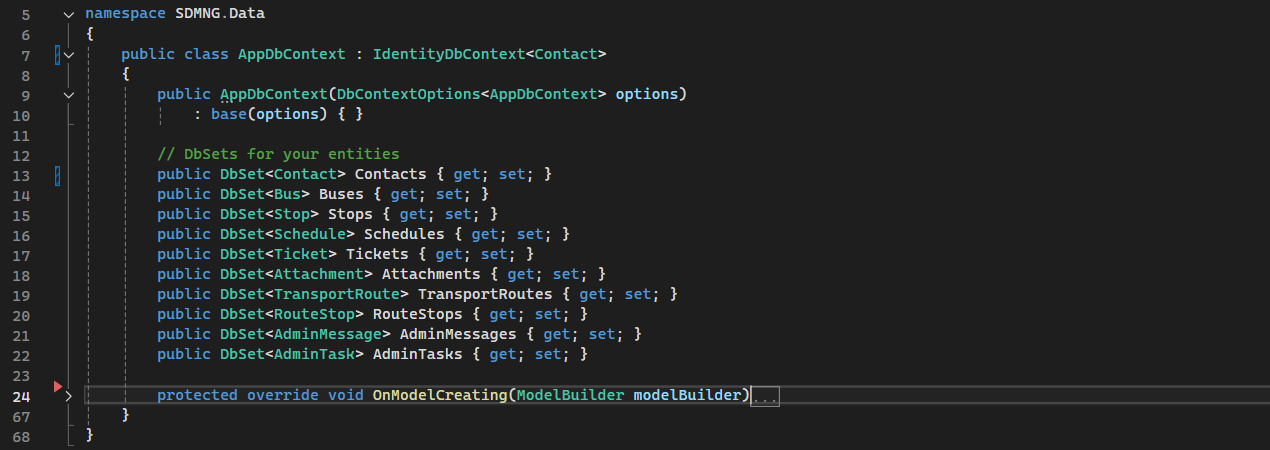
\includegraphics[width=1\textwidth]{Szakdolgozat/Mellekletek/AppDbContext.PNG}
\caption{A projektem AppDbContext osztálya látható az általam definiált modellekkel kiegészítve. }
\label{fig:appdbcontext}
\end{figure}

A \ref{fig:appdbcontext}. ábrán látható, a rendszeremben létrehozott osztályok segítségével létrehozott struktúra, amely a helyes adatbázis megvalósításában játszik kulcsszerepet. Az AppDbContext nevű osztályt az IdentityDbContext ősosztályból származtattam, majd egészítettem ki.
\vspace{\baselineskip}


Az AppDbContext osztály beállítása után szükség volt az adatbázis-fájl konfigurálására. A projekt \texttt{appsettings.json} fájlban megadtuk az adatbázis elérési útvonalát a \texttt{ConnectionStrings} szekcióban.

\begin{figure}[H]
\centering
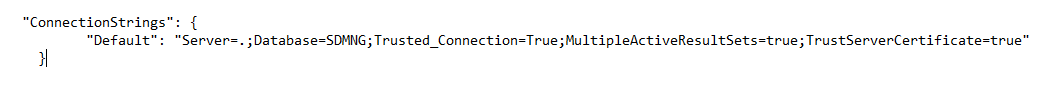
\includegraphics[width=1\textwidth]{Szakdolgozat/Mellekletek/Connectionstring.PNG}
\caption{Az adatbázis kapcsolódási kulcsa a lokális adatbázishoz.}
\label{fig:connectionstring}
\end{figure}

A \ref{fig:connectionstring}. ábrán a projektben használt \textit{connection string} látható, amely a lokális SQL Server adatbázishoz való kapcsolódást valósítja meg. Ez tartalmazza az SDMNG adatbázis elérési útvonalát, az adatbázis nevét, valamint a hitelesítési mód beállításait.
\vspace{\baselineskip}

Miután a konfigurációs fájlokat megfelelően implementáltuk, és a modellosztályaink is a tervek szerint készültek el, elérkezett az idő az első migráció létrehozására. Az adatbázis felépítését az Entity Framework migrációs rendszerével valósítottam meg. Az első migráció elkészítéséhez a terminálban a következő parancsot használtuk: dotnet ef migrations add CreateDatabase.

A parancs végrehajtása után a Migrations mappában létrejött a fentebb megadott névvel rendelkező migrációs fájl. Ezen a ponton fontos még egyszer ellenőrizni a generált adatbázis-entitásokat, és különös hangsúlyt kell fektetni a relációk helyességére. Amennyiben minden a terv szerint valósult meg, végrehajtjuk az adatbázis fizikai létrehozására vagy frissítésére szolgáló parancsot: dotnet ef database update.

Ez a parancs a korábban generált migrációs fájlok alapján felépíti vagy kiegészíti az adatbázist a megadott kapcsolati karakterlánc (connection string) segítségével.

\subsection{Vezérlők (Controllers) felépítése és működése}
Az alkalmazás működésének egyik kulcseleme a vezérlők rendszere. Ezek azok az osztályok, amelyek közvetlen kapcsolatban állnak a felhasználóval: fogadják az oldalkéréseket, előkészítik az adatokat, és eldöntik, milyen nézetet kell megjeleníteni vagy milyen műveletet kell végrehajtani. A vezérlők az MVC architektúra "C" komponensét képviselik, tehát az alkalmazás logikai magját képezik.

A projektben minden jelentősebb funkció – például jegyvásárlás, menetrendkezelés, felhasználói adatok kezelése – külön vezérlőt kapott. Ezek az osztályok a \texttt{Controllers} nevű mappában találhatóak, és  a \texttt{Controller} alaposztályból öröklődnek.

\subsubsection{A konstruktor szerepe}
A vezérlők konstruktorában történik meg az úgynevezett függőséginjektálás (dependency injection). Ez azt jelenti, hogy a vezérlő induláskor automatikusan megkapja azokat a szolgáltatásokat vagy komponenseket, amelyekre működése során szüksége lesz – például az adatbázis-kapcsolatot biztosító \texttt{AppDbContext} példányt.

\subsubsection{Aszinkron metódusok (async/await)}
A vezérlők fejlesztése során aszinkron metódusok használtam. Ennek elsődleges oka, hogy ezek a metódusok hatékonyabb működést tesznek lehetővé, különösen akkor, amikor a rendszer külső erőforráshoz – például adatbázishoz – fordul adatlekérés vagy módosítás céljából. Ilyen esetekben a programnak várnia kell a válaszra, és ha ez a várakozás egy szinkron módon írt metódusban történik, az idő alatt az egész kérés „lefagyhat”, nem képes más feladatokra reagálni.

Az aszinkron működés lényege, hogy ezek a metódusok nem akadályozzák az alkalmazás többi részének futását, miközben például háttérben adatokat kérnek le vagy dolgoznak fel. Ez különösen fontos egy webalkalmazás esetén, ahol egyszerre több felhasználói kérés is érkezhet – például jegyvásárlás, menetrend megtekintés vagy felhasználói adatok kezelése. Az \texttt{async/await} kulcsszavak használatával ezek a műveletek párhuzamosan, egymást nem akadályozva tudnak végbemenni.

Az aszinkron működés megvalósításában kulcsszerepet játszik két kifejezés: az \texttt{async} és az \texttt{await}. Az \texttt{async} kulcsszóval azt jelezzük a rendszernek, hogy az adott metódus tartalmazhat olyan műveleteket, amelyek végrehajtása hosszabb időt vesz igénybe, és ezeket érdemes nem blokkoló módon kezelni. Ezzel előkészítjük a metódust arra, hogy akár több lépésben, megszakítható módon fusson le.

Az \texttt{await} pedig azt mondja a programnak, hogy itt most egy időigényes művelet következik – például adatbázis-lekérdezés vagy fájl beolvasása –, és a vezérlés addig adódjon vissza a hívó félnek, amíg ez be nem fejeződik. A lényeg az, hogy a várakozás ideje alatt a többi feladat nem áll meg, az alkalmazás közben más kéréseket is képes kiszolgálni.

Egy-egy metódus így nemcsak hatékonyabb, de a felhasználói élményt is képes pozitívan befolyásolni, mivel csökken a válaszidő, gyorsabban jelennek meg az oldalak, és kevesebb az esély a hibákra vagy „megakadásokra”. A projekt során ezért az adatbázissal kapcsolatos lekérdezések és módosítások szinte minden esetben aszinkron módon lettek megvalósítva.

\subsubsection{Hibakeresés, csatolmánykezelés}
Az alkalmazás készítése közben nagyon fontos szerepet kapott a naplózás és a környezeti beállítások kezelése, mert ezek segítenek gyorsan megtalálni a hibákat és biztosítják, hogy a rendszer megbízhatóan működjön. A fejlesztés során az ASP.NET Core beépített \texttt{ILogger} felületét használtam, ami egy hatékony eszköz a különféle események naplózására. Ez azt jelenti, hogy az alkalmazás működésével kapcsolatos fontos információkat — például figyelmeztetéseket vagy hibákat — eltárolhatjuk, így könnyebben nyomon követhető, mi történik a háttérben, és gyorsan rá lehet jönni, ha valami nem működik jól.

Az \texttt{ILogger} segítségével például a fájlok feltöltésekor vagy e-mail küldéskor felmerülő hibák részletesen naplózhatóak, így visszakövethetővé válik, hogy mikor és milyen körülmények között jelentkezett az adott hiba. Ez különösen hasznos fejlesztési és tesztelési fázisban, amikor az alkalmazás viselkedését pontosan felügyelni kell.

A csatolmányok feltöltésekor az \texttt{IWebHostEnvironment} segítségével meghatároztam a fájlok fizikai tárolási helyét, amely általában a \texttt{wwwroot/} mappában található. Ez a megközelítés lehetővé teszi, hogy a különböző környezetekben eltérő útvonalakat használjunk, megkönnyítve ezzel a fejlesztést és a telepítést. A feltöltött fájlok elérését pedig dinamikusan, az alkalmazás futási környezetétől függően kezeljük.
\subsubsection{Regisztráció és felhaszálói szerepkör menedzselési komponensek}
A \texttt{Contact} osztályra épülő hitelesítési és regisztrációs funkciók az \texttt{AccountController} osztályon belül valósítottam meg. Ezen funkciók szétválasztását a Contact controllertől azért láttam fontosnak, mivel itt a kontakt osztály metódusai vannak definiálva a személyes fiókr nézve. A ContactControllerben viszont az admin funkciók kerültek megvalósításra az összes kontact számára. Ez jol strukturált felépítést eredményez, valamint megkönnyíti a kiegészítést, ejlesztést. 

Az \texttt{Account} vezérlő működését két fontos Identity-komponens, a \texttt{UserManager<TUser>} és a \texttt{SignInManager<TUser>} segíti. A \texttt{UserManager} az általános felhasználókezelési műveletekért felelős, mint például új felhasználó létrehozása, jelszó módosítása, szerepkörök kezelése, míg a \texttt{SignInManager} a be- és kijelentkezés lebonyolítását végzi.

A regisztráció során a rendszer egy új \texttt{Contact} példányt hoz létre a megadott adatok alapján, majd a \texttt{UserManager.CreateAsync()} metódussal menti azt az adatbázisba. A sikeres regisztrációt követően a felhasználó automatikusan hozzá van rendelve egy alapértelmezett szerepkörhöz (pl. \texttt{"User"}), amit a \texttt{UserManager.AddToRoleAsync()} metódus hajt végre. Ez lehetővé teszi a későbbi gördülékeny engedélykezelést, például admin jogosultságok bevezetését vagy jogosultságok szűrését nézetek szerint.

A bejelentkezés folyamata a \texttt{SignInManager.PasswordSignInAsync()} metódus segítségével valósul meg, amely ellenőrzi a megadott hitelesítési adatokat és elvégzi a bejelentkeztetést, ha azok helyesek. Hibás adatok esetén a rendszer visszajelzést ad a felhasználónak, ezáltal a folyamat megismétlése vagy ennek változtatásának lépése következik.

A \texttt{ChangePassword} és \texttt{VerifyEmail} akciók külön lehetőséget biztosítanak a felhasználóknak arra, hogy hitelesített módon módosítsák jelszavukat. Az e-mail cím ellenőrzését követően a jelszó eltávolítása és újra beállítása a \texttt{UserManager.RemovePasswordAsync()} és \texttt{AddPasswordAsync()} metódusokkal történik, ezzel biztosítva a jelszavak érvényességének újradefiniálását.

Végezetül a \texttt{Logout} akció gondoskodik a hitelesítési cookie érvénytelenítéséről és a felhasználó kijelentkeztetéséről a \texttt{SignInManager.SignOutAsync()} metódus segítségével, biztosítva ezzel a biztonságos felhasználói munkamenetek lezárását.

Ez a megoldás egyrészt jelentősen leegyszerűsíti a hitelesítési logika implementálását, másrészt rugalmasan bővíthető a jövőbeni funkciók igényei szerint – például kétfaktoros azonosítás, e-mail megerősítés vagy jogosultságszintek kialakítása. A \texttt{Contact} modell és a hozzá tartozó Identity szolgáltatások közösen biztosítják az alkalmazás integrált, skálázható és biztonságos felhasználókezelését.


\subsubsection{Biztonság és hitelesítés a vezérlők szintjén}
A vezérlők kialakításakor különös figyelmet fordítottam a biztonsági elvekre. Az ASP.NET Identity keretrendszer biztosította a hitelesítés és szerepkör-alapú jogosultságkezelés infrastruktúráját. Az alkalmazásban minden vezérlő és metódus, amely érzékeny adatot kezel vagy kizárólag regisztrált felhasználók számára elérhető, az \texttt{[Authorize]} attribútummal van ellátva. Egyes metódusoknál szerepkörhöz kötött elérés is alkalmazásra került, például az adminisztrációs felületek esetében kizárólag az Admin szerepkörrel rendelkező felhasználók végezhetnek műveleteket.

A \texttt{[Authorize]} attribútum legfontosabb megjelenési formája a bejelentkezés utáni jogosultság-kezelés: amennyiben a felhasználó nem azonosította magát, vagy nem rendelkezik a megfelelő szerepkörrel, nem férhet hozzá bizonyos oldalakhoz és műveletekhez. Ezáltal biztosítható, hogy például az adminisztrátor által elérhető listázási, szerkesztési vagy törlési funkciókat egy egyszerű, be nem jelentkezett felhasználó ne láthassa vagy használhassa.

A jelszavak kezelése az ASP.NET Identity rendszer beépített funkcióin keresztül történik, amely a felhasználói jelszavakat biztonságos módon, hashing algoritmus alkalmazásával tárolja az adatbázisban. A jelszavak visszafejtése nem lehetséges, csak a hash-értékek kerülnek mentésre. Ez alapértelmezett védelem a jogosulatlan hozzáférés ellen, még akkor is, ha valaki illetéktelenül hozzájutna az adatbázishoz.

\subsection{Fontosabb kontrollermetódusok megvalósítása}
\subsubsection{JegyController metódusok (Ticket)}
A fejlesztés során több olyan vezérlőmetódus készült, amelyek összetettebb funkciókat látnak el, például a jegyvásárlási folyamat kezelését. Ez magában foglalja a vásárlás rögzítését, a QR-kód generálását, valamint a felhasználó számára történő visszaigazolást e-mail formájában.

A jegyvásárlási folyamat egyik fontos lépése a QR-kód generálása, amely egy útvonalat tárol, pontosabban egy URL-t tartalmaz, amely a webalkalmazás adott oldalára — például a jegy részleteit bemutató Ticket Detail oldalra — mutat. Ez az URL tartalmazza a jegy egyedi azonosítóját, így a QR-kód beolvasásakor a felhasználó közvetlenül a megfelelő oldalra jut. A QR-kód generálása általában egy erre alkalmas, külső könyvtár vagy csomag segítségével történik, amely az URL-t vizuális, képi formátumba alakítja át (például PNG formátumú képpé), és ezt a képet az alkalmazás vagy az e-mail csatolmányaként használja fel.

Az e-mail küldése során az SMTP (Simple Mail Transfer Protocol) protokollt használjuk, amely egy széles körben elterjedt, szabványos megoldás az elektronikus levelek továbbítására. A folyamat során beállítjuk az SMTP szerver adatait, mint például a hosztnevet (pl. smtp.gmail.com), a portszámot, valamint a biztonsági protokollt (SSL vagy TLS). A hitelesítéshez szükséges a felhasználónév és az alkalmazás-specifikus jelszó, különösen ha a Gmail kétlépcsős azonosítását használjuk, mivel ilyenkor a normál jelszó nem használható az SMTP klienshez. Az e-mail összeállítása tartalmazza a címzett, a tárgy, és a levél törzsének megadását, amely akár HTML formátumban is megjelenhet, így lehetőség nyílik például a QR-kód beágyazására vagy mellékletként való csatolására. A levél elküldése aszinkron módon történik, hogy ne akadályozza a webalkalmazás egyéb működését.

A Google-fiókok biztonságos használatához ajánlott a kétfaktoros hitelesítés (2FA) beállítása, amely a jelszó mellett egy további, egyszer használatos kód megadását követeli meg. Ez a kód általában egy mobilalkalmazással, például a Google Authenticatorral generált, időalapú számsorozat, vagy SMS-ben érkező üzenet formájában érkezik. Ha 2FA engedélyezve van, az SMTP szolgáltatásokhoz nem használható a fő jelszó, ezért alkalmazás-specifikus jelszót kell létrehozni a Google fiók biztonsági beállításaiban. Ez a jelszó kizárólag az adott program vagy szolgáltatás számára érvényes, és lehetővé teszi, hogy a rendszer biztonságosan csatlakozzon az SMTP szerverhez anélkül, hogy veszélyeztetné a fiók fő jelszavát.

Ahhoz, hogy a rendszer automatikusan vissza tudjon igazolni egy sikeres jegyvásárlást e-mailben — például egy QR-kódot tartalmazó üzenet formájában — elengedhetetlen, hogy megfelelő módon előkészítsük az SMTP-alapú levélküldés technikai hátterét.

A megvalósítás egyik alapköve az, hogy az érzékeny adatokat (például az e-mail címhez tartozó hitelesítési adatokat, a kiszolgáló nevét és portját) ne kódoljuk bele az alkalmazásba, hanem külső konfigurációs fájlba konfiguráljuk, például az appsettings.json állományba. Ez nemcsak tisztább kódot eredményez, de biztonsági és karbantarthatósági szempontból is előnyös.


\subsubsection{Kapcsolatfelvétel a ContactController segítségével}

A kapcsolattartási funkció célja, hogy a felhasználók egyszerűen és gyorsan elérhessék az adminisztrátort, például kérdés, visszajelzés vagy technikai probléma esetén. Ennek megvalósításához egy űrlap áll rendelkezésre, ahol a látogató megadhatja nevét, e-mail címét, a téma tárgyát, valamint a saját üzenetét.

Az üzenet elküldése a háttérben e-mail formájában történik, az SMTP protokoll használatával. Mivel ezt a technikai megoldást korábban már részletesen bemutattam a JegyController működésénél, ahol a visszaigazolás és QR-kód küldés történt, itt csupán annak alapjaira hivatkozom. A konfigurációs részletek — például a kiszolgáló címe, portszám, hitelesítési mód, valamint az alkalmazásjelszavak és kétfaktoros azonosítás — megegyeznek az ott leírtakkal.

A különbség mindössze az üzenet tartalmában és a címzettben rejlik: míg a jegyvásárlás során egy automatikusan generált, HTML-alapú visszaigazolást küldünk ki, itt a felhasználó által kézzel írt üzenetet juttatjuk el az adminisztrátor előre meghatározott e-mail címére. Az e-mail továbbítása aszinkron módon történik, hogy ne akassza meg az alkalmazás működését.


\subsubsection{CRUD műveletek egységes megvalósítása a vezérlőkben}

A fejlesztés során az alkalmazás alapját az úgynevezett CRUD műveletek (Create, Read, Update, Delete) képezik, amelyek minden egyes entitás — legyen szó felhasználóról, jegyről, buszjáratról vagy akár kapcsolatfelvételről — kezelésének alapjai. Ezeket a funkciókat minden vezérlő (controller) esetében egységes logika mentén valósítottam meg, hogy átlátható és könnyen karbantartható struktúrát alakítsak ki.

\paragraph{Létrehozás (Create):}
Az adatok mentésének első lépése a \textit{Create} művelet, amely lehetővé teszi, hogy a felhasználó új megállót vigyen be a rendszerbe. A folyamat általában két metódusból áll: egy GET típusú lekérdezésből, amely megjeleníti az űrlapot, és egy POST típusú feldolgozásból, amely menti az adatokat.

A GET metódus célja az, hogy megjelenítse a felhasználó számára az üres űrlapot, amelyen keresztül új megálló rögzíthető. Különösen fontos ez abban az esetekben, amikor az űrlapon legördülő listákat alkalmazunk, például más entitásokkal való kapcsolat során. Ilyenkor célszerű nem az idegen kulcsot, hanem a kapcsolódó elem nevét, például az útvonal megnevezését megjeleníteni a felhasználó számára. Ehhez a GET metódus során előre le kell kérdezni a szükséges adatokat továbbítani a nézet felé. Továbbá, a GET metódus lehetőséget biztosít arra is, hogy kiszűrjük azokat az entitásokat, amelyeket már hozzárendeltünk egy másik objektumhoz. Ez különösen fontos például olyan esetekben, amikor egy buszhoz csak egyetlen sofőr rendelhető hozzá. Ebben az esetben az űrlapon csak azok a sofőrök jelennek meg a legördülő listában, akik még nincsenek hozzárendelve egyetlen buszhoz sem. Ezzel elkerülhető a többszörös hozzárendelés, és biztosítható az adatkonzisztencia.

\begin{lstlisting}
[HttpGet]
public IActionResult Create()
{
return View();
}
\end{lstlisting}

A POST metódus pedig a beküldött adatok feldolgozását végzi. A paraméterként érkező modell osztályt validálás után az adatbázisba menti. A rendszer itt egyedi azonosítót is hozzárendel a rekordhoz.

\begin{lstlisting}
[HttpPost]
[ValidateAntiForgeryToken]
public async Task Create(Stop stop)
{
stop.StopId = Guid.NewGuid().ToString();
_context.Stops.Add(stop);
await _context.SaveChangesAsync();
return RedirectToAction(nameof(Index));
}
\end{lstlisting}

A \texttt{Guid.NewGuid()} metódus gondoskodik az egyediség biztosításáról. A \texttt{Stops} tábla ezután egy új rekorddal bővül, amelyet a rendszer automatikusan ment az adatbázisba.

A legtöbb vezérlőnél — például \texttt{TicketController}, \texttt{BusController}, \texttt{ContactController} — hasonló módon történik az adatrögzítés folyamata: a GET metódus megjeleníti az űrlapot, míg a POST metódus a kitöltött adatokat dolgozza fel és menti.


\paragraph{Lekérdezés (Read):}
Az adatok megjelenítéséért felelős \textit{Read} művelet az alkalmazásban túlnyomórészt GET típusú HTTP kérések formájában valósul meg. A lekérdezések során az adatokat az Entity Framework metódusain keresztül kérdezzük le, mint például a \texttt{ToListAsync()}, \texttt{FindAsync()}, vagy a \texttt{FirstOrDefaultAsync()}.

Különösen fontos szerepet tölt be ez a művelet az adatok részletes megjelenítésében, például amikor a felhasználó meg szeretné tekinteni egy adott megálló adatait.

\begin{lstlisting}
public async Task Detail(string id)
{
if (string.IsNullOrEmpty(id)) return NotFound();

var stop = await _context.Stops
    .FirstOrDefaultAsync(s => s.StopId == id);

if (stop == null) return NotFound();

return View(stop);

}
\end{lstlisting}

Ez a metódus egy adott megálló egyedi azonosítója alapján lekérdezi az entitást az adatbázisból. A \texttt{FirstOrDefaultAsync} biztosítja, hogy vagy egy konkrét elem, vagy nulla (null) érték érkezzen vissza, ha az adott azonosítóval nem létezik megálló. A részletes nézet ezek után megjeleníti az entitás minden fontos attribútumát, például nevét, földrajzi koordinátáit és kapcsolódó elemeket.


\paragraph{Módosítás (Update):}
Az adatok frissítése általában kétlépcsős folyamatként valósul meg. Az első lépés egy GET típusú HTTP kérés, amelynek során a rendszer lekéri a módosítandó entitást, és azt egy űrlapon megjeleníti a felhasználónak. Ez lehetőséget ad az értékek szerkesztésére.

A második lépésben, POST metódus segítségével történik az új értékek mentése. A felhasználó által módosított adatokat a szerver fogadja, majd validálás után frissíti azokat az adatbázisban.

\begin{lstlisting}
[HttpPost]
[ValidateAntiForgeryToken]
public async Task Modify(string id,
[Bind("StopId,StopName,Latitude,Longitude")] Stop stop)
{
if (id != stop.StopId) return NotFound();
if (ModelState.IsValid)
{ try
    {
        _context.Update(stop);
        await _context.SaveChangesAsync();
    }
    catch (DbUpdateConcurrencyException)
    {
        if (!_context.Stops.Any(s => s.StopId == stop.StopId))
        {return NotFound();}
        throw;
    }
    return RedirectToAction(nameof(Index));
}
return View(stop);
}
\end{lstlisting}

A metódus elsőként ellenőrzi, hogy a paraméterként kapott id megegyezik-e a beküldött modell StopId értékével. Ez szükséges annak érdekében, hogy kizárjuk a tévesen átadott adatokból fakadó hibákat. Ha az azonosítók nem egyeznek, a rendszer azonnal NotFound() választ ad vissza, megszakítva a műveletet.

A ModelState.IsValid ellenőrzés során a rendszer megvizsgálja, hogy a felhasználói űrlapadatok megfelelnek-e az adott modellre vonatkozó adatintegritási és validációs szabályoknak. Csak érvényes állapot esetén hajtódik végre a frissítés.

A módosítás műveletét a context.Update() metódus végzi, amely értesíti az Entity Frameworköt arról, hogy az adott entitás állapota megváltozott. A változások tényleges mentése az adatbázisba az await \_context.SaveChangesAsync() hívással történik, amely aszinkron módon írja vissza az adatokat.

A try-catch blokk biztosítja a konkurens módosítások (concurrency) kezelését: ha például ugyanazt az entitást egy másik felhasználó időközben már frissítette vagy törölte, akkor DbUpdateConcurrencyException kivétel keletkezik. Ekkor a rendszer újraellenőrzi, hogy az adott entitás létezik-e még, és ha nem, NotFound() válasz születik.

\paragraph{Törlés (Delete):}
A törlés folyamata szintén két lépésből épül fel: egy GET típusú előkészítő műveletből, amely megerősítést kér a felhasználótól, és egy POST metódusból, amely végrehajtja az adat tényleges eltávolítását az adatbázisból.

A GET metódus célja, hogy az azonosító alapján lekérje a törölni kívánt entitást, és annak adatait megjelenítse egy megerősítő nézetben:

\begin{lstlisting}
public async Task Delete(string id)
{
if (string.IsNullOrEmpty(id)) return NotFound();

var stop = await _context.Stops
    .FirstOrDefaultAsync(s => s.StopId == id);

if (stop == null) return NotFound();

return View(stop);

}
\end{lstlisting}

A POST metódus, amelyet \texttt{DeleteConfirmed} néven definiáltunk, végzi el ténylegesen a rekord eltávolítását. Az entitást az egyedi azonosító segítségével kinyerjük, majd az Entity Framework \texttt{Remove()} metódusával töröljük.

\begin{lstlisting}
[HttpPost, ActionName("Delete")]
[ValidateAntiForgeryToken]
public async Task DeleteConfirmed(string id)
{
var stop = await _context.Stops.FindAsync(id);
if (stop != null)
{
_context.Stops.Remove(stop);
await _context.SaveChangesAsync();
}

return RedirectToAction(nameof(Index));

}
\end{lstlisting}

Ez a megoldás lehetővé teszi a biztonságos és konzisztens törlést, amely során a rendszer ellenőrzi az entitás létezését, majd a mentést követően visszairányítja a felhasználót az entitások listájához. Fontos azonban hangsúlyozni, hogy a törlés művelet implementálása során különös figyelmet kell tulajdonítani, mivel az adatok között gyakran léteznek kapcsolatok. Például ha egy megálló már hozzárendelt útvonalakban vagy menetrendekben szerepel, annak közvetlen törlése megsértheti az adatbázis integritását. Ezért célszerű az ilyen műveletek előtt ellenőrizni, hogy az adott entitás nem áll-e kapcsolatban más entitásokkal. Ha igen, akkor az adminisztrátor feladata, hogy előbb ezeket a kapcsolódó rekordokat törölje, vagy a kapcsolatok megszüntetése után hajtsa végre a törlést. A felhasználói felületen üzenetet kell megjeleníthető, amely egyértelműen jelzi, hogy az adott elem csak akkor törölhető, ha már nem szerepel más adategységekben.

\subsection{Nézetek (View) felépítése}

Az alkalmazásban a felhasználói felület megjelenítéséért az ASP.NET Core MVC nézetek (Views) felelősek, amelyek a vezérlők (Controller) által feldolgozott adatokat jelenítik meg. A nézetek szerepe, hogy az adatokat érthető és esztétikus formában mutassák be a felhasználóknak, miközben biztosítják a felhasználói interakció lehetőségét is.

A nézetek elsősorban Razor-szintaxissal készültek, amely egy egyszerű, de rugalmas eszköz az HTML és a C\# kód együttes kezelésére. Ez lehetővé teszi, hogy dinamikusan generáljuk az oldal tartalmát az adatbázisból érkező adatok alapján, miközben megőrizzük a tiszta és átlátható kódot.

A CRUD (Create, Read, Update, Delete) műveletek megvalósításához külön nézetek állnak rendelkezésre, amelyek mindegyike a megfelelő funkciót támogatja. Például a „Create” nézetben űrlapokat helyezünk el az új adatok beviteléhez, míg az „Index” vagy „List” nézet az adatbázisból lekérdezett elemek listáját jeleníti meg. A „Details” nézet egy adott elem részletes adatait mutatja be, az „Edit” pedig a módosításra szolgáló felületet biztosítja. Végül a „Delete” nézet megerősítő üzenetet jelenít meg a törlési művelet előtt.

A nézetdizájn során figyelmet fordítottam az átláthatóságra és a felhasználóbarát megjelenésre. Az alkalmazásban Bootstrap keretrendszert használtam, amely egy széles körben elterjedt CSS és JavaScript alapú eszköztár a reszponzív, modern weboldalak készítéséhez. A Bootstrap komponensek — például űrlapok, gombok, navigációs sávok és modális ablakok — segítségével egységes, könnyen kezelhető felületet sikerült kialakítani.

Az alkalmazás nézeteiben újrahasznosítható elemet alkalmaztam, mint például résznézeteket (Partial Views) és ViewComponent-eket. Ezek a komponensek lehetővé teszik, hogy az ismétlődő felhasználói felület részeket egyszer készítsük el, majd több helyen használjuk fel, ami jelentősen megkönnyíti a kód karbantartását és átláthatóságát. Különösen a felhasználói hitelesítéshez kapcsolódó oldalak, mint a bejelentkezés és regisztráció, a .NET Identity keretrendszer szolgáltatásaira épülnek. Ezeknél a funkcióknál résznézeteket használtam a vizuális elemek szervezésére, így egységes megjelenést és egyszerűbb kezelhetőséget biztosítva az autentikációs folyamatokhoz.

\subsection{Főbb Nézetek}
\subsubsection{Navigációs sáv és legördülő menü }
A webalkalmazás felhasználói felületének egyik központi eleme a navigációs sáv, amelynek megjelenése dinamikusan igazodik a felhasználó jogosultsági szintjéhez. A sáv alapértelmezetten tartalmazza azokat a menüpontokat, amelyek minden látogató – akár be nem jelentkezett felhasználó – számára elérhetők. Ilyen például a megállók (Stations), az útvonalak (Routes), a menetrendek (Schedules), a saját jegyek (My Tickets), valamint az ügyfélszolgálati kapcsolatfelvétel (Contact us) lehetősége. Ezek a funkciók elsősorban információs célokat szolgálnak, és biztosítják, hogy az alkalmazás alapvető szolgáltatásai mindenki számára hozzáférhetőek legyenek.

A rendszer ezen felül támogatja a szerepkör-alapú hozzáférést is, amelynek eredményeként bizonyos menüpontok kizárólag az adminisztrátori jogosultsággal rendelkező felhasználók számára válnak láthatóvá. Amennyiben a rendszer érzékeli, hogy a bejelentkezett felhasználó az „Admin” szerepkörhöz tartozik, egy további legördülő menü is megjelenik a navigációs sávban. Ez a menü – „Management” néven – olyan adminisztratív funkciókat tartalmaz, amelyek segítségével az adminisztrátor kezelheti a buszokat, megállókat, jegyeket, útvonalakat, menetrendeket, felhasználói kapcsolatokat, csatolmányokat, jogosultságokat, valamint a rendszerben beérkezett üzeneteket és a belső teendőlistát is. Minden egyes menüpont mögött egy adott kontrollerhez és akciómetódushoz tartozó hivatkozás található, amelyek az ASP.NET MVC keretrendszer segítségével biztosítják a navigációt az adminisztratív oldalak felé.

A menüelemek megjelenését a rendszer a User.IsInRole("Admin") feltétel alapján szabályozza, így a jogosultsággal nem rendelkező felhasználók számára ezek az elemek teljes mértékben rejtve maradnak. Ez nemcsak a biztonság szempontjából előnyös, hanem a felhasználói felület letisztultságát is biztosítja.

A navigációs sáv jobb oldalán helyezkedik el az azonosítási rész, amely be nem jelentkezett állapotban a bejelentkezés („Login”) és a regisztráció („Register”) lehetőségét kínálja, míg bejelentkezett felhasználók esetén a felhasználó nevét és a kijelentkezési („Logout”) opciót jeleníti meg. Ez a megoldás lehetővé teszi, hogy az alkalmazás mindig az aktuális felhasználó státuszának megfelelő kezelőfelületet biztosítson.

A webalkalmazás fejléce egy Bootstrap alapú navigációs sávval valósul meg, amelyet a \texttt{.cshtml} nézetfájlban Razor szintaxissal kombinálva hoztunk létre. A \texttt{<nav>} elem a sáv keretét adja, amely kis képernyőn összehúzható, nagyobb felületen pedig automatikusan szélesedik.

A tartalom a \texttt{<div class="container-fluid">} blokkban helyezkedik el, amely teljes szélességet biztosít az elrendezéshez. A bal oldalon található a \texttt{<a class="navbar-brand">} elem, amely az alkalmazás logójaként szolgál, és a főoldalra navigál a megadott \texttt{asp-controller} és \texttt{asp-action} attribútumok segítségével.

A menüpontokat egy \texttt{<ul class="navbar-nav">} lista tartalmazza, amely rugalmasan kitölti a rendelkezésre álló helyet. Ezen belül a kód egy feltételes blokkot tartalmaz, amely kizárólag akkor hajtódik végre, ha az aktuális felhasználó rendelkezik az „Admin” szerepkörrel. Ezt a Razor \texttt{User.IsInRole("Admin")} feltétele vezérli. Ha a feltétel igaz, megjelenik egy legördülő menü „Management” néven, amely különböző adminisztratív funkciókhoz tartozó hivatkozásokat tartalmaz.

Ezek a hivatkozások a különböző kontrollerek \texttt{Index} metódusaira mutatnak, például a buszok, megállók, jegyek, útvonalak, csatolmányok, menetrendek vagy jogosultságok kezelésére szolgáló oldalakra. Minden menüpont egyedi ikonokkal van ellátva a felhasználói élmény érdekében, amelyet a Bootstrap Icons könyvtár biztosít.

A legördülő menü alatt, az admin jogkörrel nem rendelkező felhasználók számára is elérhető elemek következnek. Ezek között szerepelnek a megállók (\texttt{Stations}), útvonalak (\texttt{Routes}), menetrendek (\texttt{Schedules}), saját jegyek (\texttt{My Tickets}) és az ügyfélszolgálattal való kapcsolatfelvételi lehetőség (\texttt{Contact us}). Ezek a hivatkozások a látogatók számára biztosítanak alapvető funkcionalitást, függetlenül a bejelentkezési állapottól.

A navigációs sáv jobb oldalán egy külön szeparált résznézet, a \texttt{\_LoginPartial}, jelenik meg, amely felelős a felhasználó hitelesítési állapotának megjelenítéséért. Ez a rész automatikusan alkalmazkodik az aktuális felhasználó állapotához: amennyiben a látogató még nem jelentkezett be, a felület a „Login” és „Register” lehetőségeket kínálja. Ezzel szemben bejelentkezett felhasználó esetén megjelenik a felhasználónév, valamint a „Logout” gomb, amely lehetőséget biztosít a kijelentkezésre.

A résznézet (\emph{partial view}) használata itt nemcsak kényelmi szempontból előnyös, hanem fejlesztői szempontból is számos haszonnal jár. Egyrészt elkülöníti a hitelesítéssel kapcsolatos logikát a fő nézettől, így biztosítva a kód átláthatóságát. Másrészt lehetővé teszi, hogy ezt a funkcionalitást újra felhasználjuk több helyen is az alkalmazásban, például különböző elrendezési sablonokban vagy specifikus nézetekben. Így, ha a jövőben módosítani szükséges a bejelentkezéshez vagy kijelentkezéshez kapcsolódó felületet, elegendő csak a \texttt{\_LoginPartial.cshtml} fájlt frissíteni, és az automatikusan érvényesül minden olyan nézetben, ahol ez a résznézet be van ágyazva.

\begin{figure}[H]
\centering

\includegraphics[width=1\textwidth]{Szakdolgozat/Mellekletek/navsavlogin1.PNG}
\caption{A navigációs sáv megjelenése bejelentkezett adminisztrátor számára.}
\label{fig:navsavlogged}
\end{figure}

A \ref{fig:navsavlogged}. ábrán a navigációs sáv bejelentkezett állapotban látható, adminisztrátori jogosultság mellett. Ebben az esetben a felhasználó számára elérhetővé válik egy további, legördülő menü, amely az adminisztrációs funkciókat csoportosítja. A menü tartalmazza többek között a megállók (Stops), buszok (Buses), útvonalak (Routes), menetrendek (Schedules), csatolmányok (Attachments), felhasználók (Contacts), jogosultságok (Roles), valamint teendők (ToDo List) kezelésére szolgáló linkeket. Ezek a nézetek csak az adminisztrátor szerepkörrel rendelkező felhasználók számára jelennek meg, és lehetőséget biztosítanak az alkalmazás teljes körű adatkezelésére és adminisztrálására. A menüsáv jobb oldalán továbbra is elérhető a kijelentkezési lehetőség, amely biztosítja a munkamenet megfelelő lezárását.

\subsubsection{Felhasználókezelési nézetek és résznézetek alkalmazása}

Az alkalmazásban a felhasználói azonosítással kapcsolatos funkciók – például a bejelentkezés, regisztráció, jelszócsere vagy email-ellenőrzés – dedikált nézeteken keresztül valósulnak meg, amelyek az \texttt{AccountController} vezérlőhöz kapcsolódnak. Ezek a nézetek a háttérben, ahogy már fentebb is említettem, a \texttt{Contact} nevű egyedi felhasználói modell adataira épülnek, amely az ASP.NET Identity \texttt{IdentityUser} osztályából származik.

A nézetek mindegyike külön ViewModel-t használ az űrlapadatok átadásához és validálásához. A \texttt{LoginViewModel}, \texttt{RegisterViewModel}, \texttt{VerifyEmailViewModel} és \texttt{ChangePasswordViewModel} mind külön-külön reprezentálják az adott funkcióhoz szükséges adatokat és a mezőkhöz kapcsolódó ellenőrzési szabályokat. A Razor-alapú nézetekben az \texttt{asp-for} és \texttt{asp-action} attribútumok biztosítják az adatkötést, valamint az automatikus hivatkozást a vezérlő megfelelő metódusaihoz.

Minden oldal egységes elrendezést követ, amelyet a \texttt{\_AccountLayout.cshtml} nézet biztosít. Ez a sablon definiálja az általános megjelenést, amelyet az összes hitelesítéssel kapcsolatos nézet örököl. Az űrlapok végén található \texttt{@section Scripts} blokk aszinkron módon betölti a \_ValidationScriptsPartial.cshtml nevű résznézetet, amely a kliensoldali validáláshoz szükséges JavaScript-függvényeket tartalmazza. Ennek köszönhetően a felhasználó azonnali visszajelzést kap a hibásan kitöltött vagy hiányzó mezőkről, még az adatküldés előtt.

Külön figyelmet érdemel a \texttt{\_LoginPartial.cshtml} résznézet szerepe, amely nem a hitelesítési nézeteken belül, hanem a főoldal elrendezésében, a navigációs sáv jobb oldalán jelenik meg. Ez a rész automatikusan lekérdezi a felhasználó hitelesítési állapotát, és dinamikusan változtatja a megjelenített tartalmat, amennyiben a látogató nincs bejelentkezve, megjelennek a „Login” és „Register” hivatkozások; ha viszont a felhasználó azonosítva van, akkor a felhasználónevet, valamint a kijelentkezési lehetőséget jeleníti meg.


\vspace{\baselineskip}
\subsubsection{Lista oldalak}
A listanézetek felépítése egységes, ahol az adott entitáshoz tartozó legfontosabb adatokat oszlopokban mutatjuk be. Minden ilyen nézet tartalmaz egy „Actions” nevű oszlopot is, amelyben három alapvető művelet található: a részletek megtekintése (Detail), az adat módosítása (Modify/Edit), valamint az elem törlése (Delete). Ezek a gombok minden egyes listaelem mellett megjelennek, és mindegyikhez az adott elem egyedi azonosítója (ID) van hozzárendelve. Ennek köszönhetően, amikor egy felhasználó rákattint valamelyik művelet gombra, a sornak vagy elemnek megfelelő oldalt nyitja meg, így biztosítva a pontos és gyors navigációt az funkciókat megvalósító oldalak között.

Az adminisztrátori feladatok kezelésére szolgáló nézet egy egyszerű táblázatos elrendezést használ, amely a \texttt{List<AdminTask>} típusú modell alapján jeleníti meg a rendszerben rögzített teendőket. A nézet elején a \texttt{@model} direktíva határozza meg, hogy milyen típusú adatot vár a nézet – jelen esetben az \texttt{AdminTask} típusú objektumokat tartalmazó listát.

A fejlécként szolgáló \texttt{ViewData["Title"]} meghatározza a lap címét, amely az oldal HTML fejlécében is megjelenik. Ezt követi egy főcím, valamint egy gomb a feladatok létrehozására (\texttt{Create}), amely egy \texttt{asp-action} segítségével a létrehozó űrlapra irányítja a felhasználót.

A feladatokat egy Bootstrap-alapú táblázat (\texttt{<table class="table">}) jeleníti meg. A \texttt{<thead>} rész a táblázat oszlopcímeit tartalmazza, amelyek sorrendben a feladat teljesítettségét jelző ikon, a cím, a határidő és a hozzárendelt műveletek.

A \texttt{<tbody>} részben egy \texttt{@foreach} ciklus segítségével iterálunk végig a modell objektumain. Minden egyes \texttt{AdminTask} típusú elem egy táblázatsorban (\texttt{<tr>}) kerül megjelenítésre. Az adott sor háttérszíne dinamikusan módosul: amennyiben a feladat már el van végezve (\texttt{IsResolved = true}), a sor \texttt{table-success} osztályt kap, ami zöld hátteret biztosít.

Az első oszlopban egy ikon jelenik meg, amennyiben a feladat már teljesített. Ez a Bootstrap Icons könyvtárból származik, és vizuálisan is jelzi az állapotot (\texttt{bi-check-circle-fill}). A második oszlop a feladat címét (\texttt{Title}), míg a harmadik a határidőt (\texttt{DueUntil}) jeleníti meg, rövid dátumformátumban.

Az utolsó oszlopban két gomb található: a „Details” gomb egy részletes nézetre navigál az adott feladattal kapcsolatban, míg az „Edit” gomb a módosító űrlaphoz visz. Mindkét hivatkozás dinamikusan kapja meg a feladat azonosítóját (\texttt{Id}) az \texttt{asp-route-id} attribútumon keresztül.

Ez a megközelítés nemcsak az adminisztratív feladatok kezelésére használható, hanem bármely entitástípus (például jegyek, útvonalak, felhasználók, csatolmányok) listázására is alkalmas. 


\subsubsection{Térképes megjelenítés a Stop részletező nézetben}
A megállók részletező nézete a felhasználói felület egyik kulcseleme, amely nemcsak szöveges információt nyújt a kiválasztott megállóról, hanem vizuálisan is segíti a tájékozódást egy interaktív térkép segítségével. A felület célja, hogy a felhasználó könnyen és gyorsan át tudja tekinteni egy adott megálló legfontosabb adatait, illetve annak pontos földrajzi elhelyezkedését.

A nézet az adott megálló objektum adatait jeleníti meg, amely a rendszerben egy Stop típusú modellként van definiálva. A megjelenített mezők közé tartozik a megálló neve, valamint annak szélességi és hosszúsági koordinátái. Ezek az értékek olvasható, de nem szerkeszthető formában jelennek meg, hogy a felhasználó ne tudjon véletlenül módosítani rajtuk.

A nézet különlegessége a térképes megjelenítés, amely a Leaflet nevű JavaScript-alapú térképkönyvtárra épül. Ez a könyvtár lehetővé teszi, hogy egy egyszerű, mégis interaktív térképet helyezzünk el az oldalon. A térkép automatikusan a kiválasztott megálló koordinátáira fókuszál, és egy jelölőt (marker) is elhelyez rajta, amely rámutat a pontos helyszínre. A jelölő fölé egy információs ablak is megnyílik, amelyben a megálló neve szerepel.

A megálló adatlap nézetében egy JavaScript-alapú megoldás jeleníti meg a megálló földrajzi elhelyezkedését térképen. Ennek célja, hogy a felhasználó pontosan lássa, hol található az adott megálló. A megvalósítás alapja az, hogy az adatmodellből (`Stop`) származó földrajzi koordináták (szélesség és hosszúság) JavaScript változókba kerülnek:

\begin{lstlisting}[language=JavaScript]
var lat = @Html.Raw(Model.Latitude.ToString().Replace(',', '.'));
var lng = @Html.Raw(Model.Longitude.ToString().Replace(',', '.'));
\end{lstlisting}

Ez a lépés biztosítja, hogy a .NET-ben használt tizedesvesszők megfelelően átalakuljanak tizedespontokká, amelyeket a JavaScript értelmezni tud. Ezt követően egy egyszerű ellenőrzés biztosítja, hogy a koordináták érvényes számok:

\begin{lstlisting}[language=JavaScript]
if (!isNaN(lat) && !isNaN(lng)) {
\end{lstlisting}

Ha az értékek helyesek, létrejön a térképobjektum. A térkép a HTML oldalon definiált \texttt{<div>} elemre (`id="stopMap"`) kerül:

\begin{lstlisting}[language=JavaScript]
var map = L.map('stopMap').setView([lat, lng], 15);
\end{lstlisting}

Ezután hozzáadjuk a térkép vizuális rétegét, az úgynevezett csemperéteget az OpenStreetMap szolgáltatásból:

\begin{lstlisting}[language=JavaScript]
L.tileLayer('https://{s}.tile.openstreetmap.org/{z}/{x}/{y}.png', {
    maxZoom: 18
}).addTo(map);
\end{lstlisting}

A megálló pontos helyét egy markerrel jelöljük, amelyhez egy információs buborék is társul, amely automatikusan megnyílik, amint betöltődik a térkép:

\begin{lstlisting}[language=JavaScript]
L.marker([lat, lng])
    .addTo(map)
    .bindPopup("<strong>@Model.StopName</strong>")
    .openPopup();
\end{lstlisting}

A megálló adatlapján megjelenő térképes komponens kulcsfontosságú felhasználói élményt nyújt, mivel lehetővé teszi a megálló földrajzi helyének közvetlen, vizuális azonosítását. A rendszer nem csupán a megálló nevét és koordinátáit jeleníti meg szövegesen, hanem automatikusan betölt egy interaktív térképet is, amely a megálló pontos pozíciójára fókuszál. Ezt a térképet automatikusan egy előre definiált nagyítási szinten nyitja meg a rendszer, így a felhasználó azonnal az adott megálló szűk környezetét látja – például az utcát, csomópontot vagy városrészt, ahol az elhelyezkedik.

Ennek a megközelítésnek az egyik legnagyobb előnye, hogy a felhasználónak nem szükséges a megálló nevét külső alkalmazásban, például térképszolgáltatóban újra beírnia vagy külön keresnie. A rendszer tehát nem hagyatkozik arra, hogy a név alapján a felhasználó majd önállóan beazonosítja a megállót, hanem maga szolgáltatja a térképes, hajszálpontos helyadatot. Ez a megoldás jelentősen csökkenti az eltévedés vagy félreértés kockázatát, különösen akkor, ha több hasonló nevű megálló is létezik egy városon belül.

\subsubsection{Útvonal részletező nézet – több megálló vizuális megjelenítése térképen}

Az útvonal nézet működésében több ponton is párhuzamba állítható a megálló részletező felülettel: itt is térképes megjelenítés segíti a felhasználót, viszont a fókusz már nem egyetlen helyszín bemutatásán van, hanem egy egész megállósorozat áttekintésén. A nézet célja, hogy az útvonalhoz tartozó állomásokat sorrendben és valós helyükön mutassa be, azokat a térképen vizuálisan összekötve. Ezáltal a felhasználó nemcsak név szerint keresheti ki az egyes megállókat, hanem egy teljes képet kap arról, hogyan épül fel az adott útvonal.

A rendszer minden megállóhoz egy-egy \texttt{marker} objektumot rendel, amelyet a térképen elhelyez. Ezeket JavaScript segítségével dolgozza fel, a koordináták alapján. Minden pont bekerül egy \texttt{waypoints} nevű tömbbe is, amelyet később a térképútvonal-rajzolás során használunk.

\begin{lstlisting}
var marker = L.marker([lat, lng]).addTo(map).bindPopup(stopName);
waypoints.push(L.latLng(lat, lng));
\end{lstlisting}

Miután az összes megálló feldolgozásra került, az útvonal kirajzolása a Leaflet Routing Machine nevű bővítmény segítségével történik. Ez a könyvtár a megadott pontokat vonalakkal köti össze, sorrendben:

\begin{lstlisting}
L.Routing.control({
    waypoints: waypoints,
    lineOptions: {
        styles: [
            { color: '#FF1493', weight: 6, opacity: 0.95 },
            { color: '#FFFFFF', weight: 2, opacity: 1 }
        ]
    },
    createMarker: function() { return null; },
    routeWhileDragging: false
}).addTo(map);
\end{lstlisting}

A \texttt{lineOptions} szekció a vonal stílusáért felel, így az jól elkülönül más térképi elemektől. A \texttt{createMarker: function() \{ return null; \}} sor azért került be, hogy az útvonal-vezérlő ne helyezzen el újabb alapértelmezett jelölőket, mivel azt már korábban megtettük kézzel.

A térkép végül automatikusan a teljes útvonalra igazítja a nézetet, az összes megállót figyelembe véve:

\begin{lstlisting}
map.fitBounds(L.latLngBounds(waypoints));
\end{lstlisting}

Ez a térképes funkció hasonló célt szolgál, mint a megálló nézetben látott statikus marker, ugyanakkor ennél összetettebb élményt nyújt: nem egyetlen pontot, hanem egy útvonal teljes struktúráját jeleníti meg. A felhasználónak így nem kell találgatnia, hogy merre halad az adott járat – a rendszer megmutatja, pontról pontra, vizuálisan is.


\subsubsection{Ticket detail page }

A jegyrészletező oldal a projekt szempontjából kiemelt jelentőséggel bír, hiszen ez az a funkció, amely az egész alkalmazás ötletét elindította. A kezdeti elképzelés abból született, hogy a felhasználók számára egy olyan felületet biztosítsunk, ahol a megvásárolt jegyük minden lényeges információja egyetlen, jól átlátható nézetben elérhető.

Az oldal célja, hogy minden olyan információt tartalmazzon, ami az utazás szempontjából fontos lehet. Megjelenik rajta a járat neve, az ahhoz tartozó busz rendszáma, a lefoglalt ülőhely száma, valamint az indulási és érkezési időpontok, illetve azok helyszínei. Ezen adatok strukturált formában kerülnek megjelenítésre, így a felhasználó egy pillantással át tudja tekinteni a foglalás részleteit.

Ami azonban igazán megkülönbözteti ezt a felületet más rendszerektől, az a térképes integráció. A nézet közvetlenül tartalmazza az utazás útvonalát is, amely egy térképen jelenik meg, vizuálisan kirajzolva a megállók közötti kapcsolatokat. Ennek óriási előnye, hogy a felhasználónak nem kell külön oldalakon keresgélnie, vagy új ablakot megnyitnia annak érdekében, hogy földrajzi képet kapjon az útvonalról – az interaktív térkép közvetlenül a jegyadatok mellett helyezkedik el, így a kétféle információ egy helyen, egymást kiegészítve jelenik meg.

Ez a megközelítés nemcsak kényelmi szempontból előnyös, hanem a felhasználói élmény szempontjából is kulcsfontosságú. A rendszer úgy lett kialakítva, hogy a legfontosabb információkat – akár időbeli, akár térbeli adatokról legyen szó – egyetlen oldalon tegye elérhetővé, ezzel is minimalizálva a felesleges navigációt és az információk keresésére fordított időt. Mindez nem csupán praktikus, hanem szemléletformáló is: a projekt középpontjába magát az utazó embert helyezi, és a lehető legkényelmesebb módon szolgáltatja számára a szükséges adatokat.

\begin{figure}[H]
    \centering
    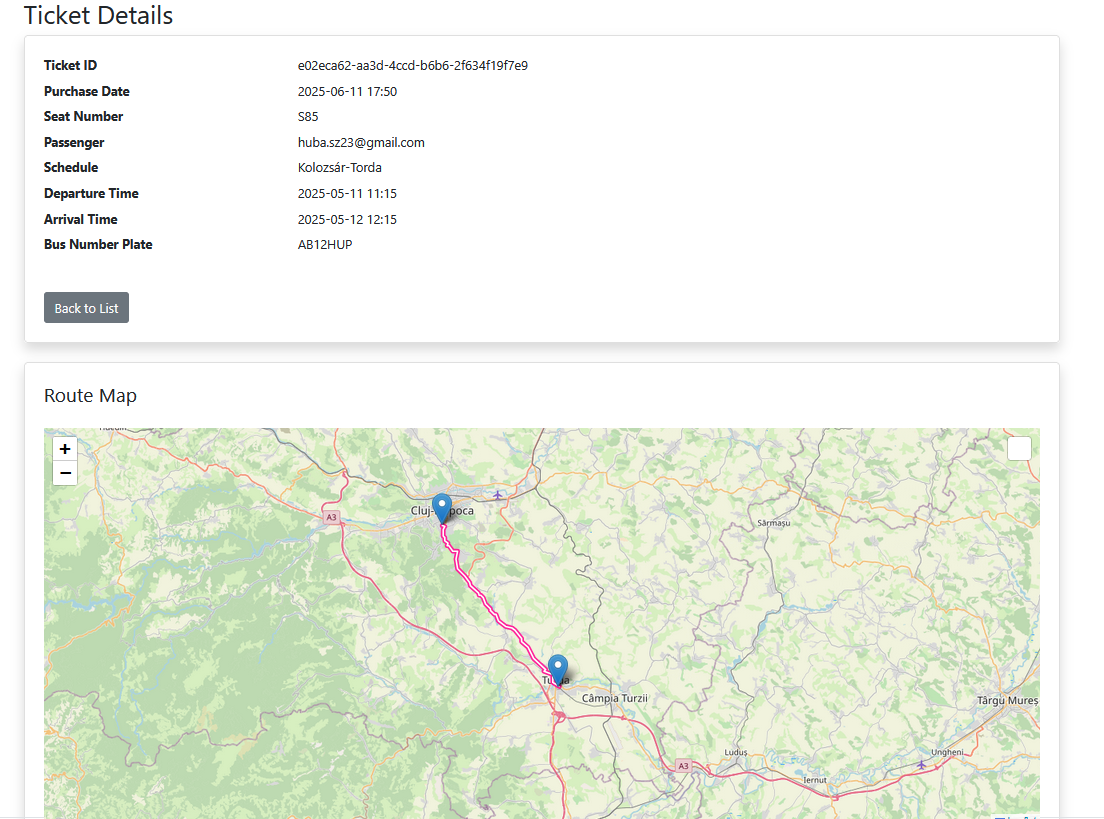
\includegraphics[width=0.9\textwidth]{Szakdolgozat/Mellekletek/ticketdetail.PNG}
    \caption{Példa: egy Kolozsvár–Torda útvonalra vásárolt jegy részletező nézete. Az oldalon jól látható a járat neve, a busz rendszáma, az ülőhely száma, az indulási és érkezési időpontok és helyszínek, valamint a teljes útvonal térképes megjelenítése.}
    \label{fig:ticket-detail-kolozsvar-torda}
\end{figure}







\end{document}
